\documentclass[12pt,addpoints]{repaso2}
\grado{2}
\nivel{Secundaria}
\cicloescolar{2026-2027}
\materia{Matemáticas}
\unidad{1}
\title{Repaso Extraordinario}
\aprendizajes{
      \item Resuelve problemas que impliquen la suma, resta, la multiplicación y la división de números enteros, aplicando las reglas correspondientes.
      \item Identifica y ubica números negativos en una recta numérica, comparando su magnitud.
      \item Aplica las propiedades de las potencias a números negativos en la resolución de problemas.
      \item Resuelve problemas que involucren las leyes de los exponentes, y expresa números en notación científica.
      \item Resuelve problemas de contexto científico y tecnológico utilizando la notación científica.
      \item Identifica y ubica puntos en el plano cartesiano, y comprende la estructura de los cuadrantes.
      \item Calcula la pendiente de una recta y comprende su significado en diferentes contextos.
      \item Resuelve problemas que involucren el uso de porcentajes, mediante la ``regla de tres''.
}
\author{Melchor Pinto, J.C.}
\begin{document}
\INFO%
\newpage
\begin{multicols}{2}
	\tableofcontents
\end{multicols}
\newpage
\begin{questions}
\section{Unidad 1}
	\subsection{Cálculos numéricos}
	\subsubsection{Suma de números}
	\questionboxed[1]{Realiza las siguientes \emph{sumas}:

		\begin{parts}
			\begin{multicols}{3}
				\part $321+51+134=$ \fillin[$506$][0in]

				\part $0.1+0.02+0.03+0.4=$ \fillin[$0.55$][0in]
				
				\part \ifprintanswers{\opadd[hfactor=decimal,resultstyle=\color{red},carryadd=true]{40602}{389603}}
				\else{$40602+389603=$}\fi


								\columnbreak%

				\part \ifprintanswers{\opadd[hfactor=decimal,resultstyle=\color{red},carryadd=true]{67.54}{564.073}}
				\else{$67.54+564.073=$}\fi

				\part \ifprintanswers{\opadd[hfactor=decimal,resultstyle=\color{red},carryadd=true]{1248.97}{46.5}}
				\else{$1248.97+46.5=$}\fi


				\part \ifprintanswers{\opadd[hfactor=decimal,resultstyle=\color{red},carryadd=true]{5423.3}{32140}}
				\else{$5423.3+32140=$}\fi

								\columnbreak%

				\part \ifprintanswers{\opadd[hfactor=decimal,resultstyle=\color{red},carryadd=true]{3440.64}{280.79}}
				\else{$3440.64+280.79=$}\fi

				\part \ifprintanswers{\opadd[hfactor=decimal,resultstyle=\color{red},carryadd=true]{67.67}{502.907}}
				\else{$67.67+502.907=$}\fi


				\part \ifprintanswers{\opadd[hfactor=decimal,resultstyle=\color{red},carryadd=true]{5740.504}{109.23}}
				\else{$5740.504+109.23=$}\fi

				
			\end{multicols}
		\end{parts}
	}

	\subsubsection{Resta de números}

	\questionboxed[1]{Realiza las siguientes \emph{restas}:

		\begin{parts}
			\begin{multicols}{3}
				\part \ifprintanswers{   \opsub[hfactor=decimal,resultstyle=\color{red},carryadd=true,carrysub=true]{82.48}{28.19} }
				\else{$82.48-28.19=$}\fi

				\part \ifprintanswers{   \opsub[hfactor=decimal,resultstyle=\color{red},carryadd=true,carrysub=true]{495}{92} }
				\else{$495-92=$}\fi

				\part \ifprintanswers{   \opsub[hfactor=decimal,resultstyle=\color{red},carryadd=true,carrysub=true]{937}{682} }
				\else{$937-682=$}\fi

				\part \ifprintanswers{   \opsub[hfactor=decimal,resultstyle=\color{red},carryadd=true,carrysub=true]{341}{212} }
				\else{$341-212=$}\fi

				\part \ifprintanswers{   \opsub[hfactor=decimal,resultstyle=\color{red},carryadd=true,carrysub=true]{465.76}{292.41} }
				\else{$465.76-292.41=$}\fi

				\part \ifprintanswers{   \opsub[hfactor=decimal,resultstyle=\color{red},carryadd=true,carrysub=true]{762}{394} }
				\else{$762-394=$}\fi

				\part \ifprintanswers{   \opsub[hfactor=decimal,resultstyle=\color{red},carryadd=true,carrysub=true]{850}{472} }
				\else{$850-472=$}\fi

				\part \ifprintanswers{   \opsub[hfactor=decimal,resultstyle=\color{red},carryadd=true,carrysub=true]{945}{173} }
				\else{$945-173=$}\fi

				\part \ifprintanswers{   \opsub[hfactor=decimal,resultstyle=\color{red},carryadd=true,carrysub=true]{0.1}{0.02} }
				\else{$0.1-0.02=$}\fi
			\end{multicols}
		\end{parts}
	}

	\subsubsection{Multiplicación de números}

	\questionboxed[1]{Realiza las siguientes \emph{multiplicaciones}:

		\begin{parts}
			\begin{multicols}{4}
				\part \ifprintanswers{\opmul[resultstyle=\color{red},displayintermediary=None]{865}{7} }
				\else{\opmul[resultstyle=\color{white},displayintermediary=None]{865}{7}}\fi

				\part \ifprintanswers{\opmul[resultstyle=\color{red},displayintermediary=None]{57}{10.34} }
				\else{\opmul[resultstyle=\color{white},displayintermediary=None]{57}{10.34}}\fi\\[0.5em]

				\part \ifprintanswers{\opmul[resultstyle=\color{red},displayintermediary=None]{284}{8} }
				\else{\opmul[resultstyle=\color{white},displayintermediary=None]{284}{8}}\fi

				\part \ifprintanswers{\opmul[resultstyle=\color{red},displayintermediary=None]{24.13}{15} }
				\else{\opmul[resultstyle=\color{white},displayintermediary=None]{24.13}{15}}\fi\\[0.5em]

				\part \ifprintanswers{\opmul[resultstyle=\color{red},displayintermediary=None]{26.37}{9} }
				\else{\opmul[resultstyle=\color{white},displayintermediary=None]{26.37}{9}}\fi

				\part \ifprintanswers{\opmul[resultstyle=\color{red},displayintermediary=None]{1851}{21} }
				\else{\opmul[resultstyle=\color{white},displayintermediary=None]{1851}{21}}\fi\\[0.5em]

				\part \ifprintanswers{\opmul[resultstyle=\color{red},displayintermediary=None]{411}{4} }
				\else{\opmul[resultstyle=\color{white},displayintermediary=None]{411}{4}}\fi

				\part \ifprintanswers{\opmul[resultstyle=\color{red},displayintermediary=None]{515}{37} }
				\else{\opmul[resultstyle=\color{white},displayintermediary=None]{515}{37}}\fi\\[0.5em]
			\end{multicols}
		\end{parts}
	}

	\subsubsection{División de números}

	\questionboxed[1]{Calcula el \textbf{cociente} y el \textbf{residuo} de las siguientes \emph{divisiones}:

		\begin{parts}
			\begin{multicols}{3}
				\part $785 \divisionsymbol 125=$ \\[0.5em]
				Cociente: \fillin[6][0in]\\
				Residuo: \fillin[35][0in]\\

				\part $655.23 \divisionsymbol 23=$ \\[0.5em]
				Cociente: \fillin[28][0in]\\
				Residuo: \fillin[11][0in]\\

				\part $123 \divisionsymbol 1.2=$ \\[0.5em]
				Cociente: \fillin[102][0in] \\
				Residuo: \fillin[6][0in]\\

				\part $723 \divisionsymbol 8=$ \\[0.5em]
				Cociente: \fillin[90][0in]\\
				Residuo: \fillin[3][0in]\\

				\part $90 \divisionsymbol 21=$ \\[0.5em]
				Cociente: \fillin[4][0in]\\
				Residuo: \fillin[6][0in]\\

				\part $22 \divisionsymbol 0.2=$ \\[0.5em]
				Cociente: \fillin[110][0in]\\
				Residuo: \fillin[0][0in]\\
			\end{multicols}
		\end{parts}
	}

	\subsubsection{Resolución de problemas}

	\questionboxed[1]{Resuelve los siguientes problemas:

		\begin{parts}
			\begin{multicols}{2}
				\part Una computadora tiene un disco duro de 368 GB de memoria, si varios programas ocupan 128.75 GB. ¿Qué cantidad de memoria está libre?

				\begin{solutionbox}{1.2cm}
					$368-128.75=$ \fillin[$239.25$][0in]
				\end{solutionbox}

				\part En un estacionamiento conté 57 automóviles, 31 camionetas y 23 taxis, ¿cuántos vehículos había en total?

				\begin{solutionbox}{1.2cm}
					$57+31+23=$ \fillin[$111$][0in]
				\end{solutionbox}

				\part El precio de 385 artículos comerciales es de 1232 pesos. ¿Cuál es el precio unitario de cada artículo?

				\begin{solutionbox}{1.2cm}
					$1232 \divisionsymbol 385=$ \fillin[$3.20$][0in]
				\end{solutionbox}
				
				\part Las ventas de boletos que registra un cine en un fin de semana son las siguientes: 490 boletos vendidos el viernes, 780 el sábado y 1234 el domingo. ¿Cuántos boletos se vendieron en total?
				
				\begin{solutionbox}{1.2cm}
					$490+780+1234=$ \fillin[$2504$][0in]
				\end{solutionbox}

				\part Una pintura tiene un costo de 25.75 pesos el litro, una persona compra 48 litros. ¿Cuánto debe pagar?
			
				\begin{solutionbox}{1.2cm}
					$25.75 \times 48=$ \fillin[$1236$][0in]
				\end{solutionbox}
			
				\part Un elástico se estira tres veces su longitud en su estado normal. Si mide 5.23 cm en su estado normal, ¿cuántos centímetros alcanza al ser estirado?
			
				\begin{solutionbox}{1.2cm}
					$5.23 \times 3=$ \fillin[$15.69$][0in]
				\end{solutionbox}

				\part Si un dólar equivale a 19 pesos. ¿Cuántos pesos equivaldrán 615 dólares?
			
				\begin{solutionbox}{1.2cm}
					$19 \times 615=$ \fillin[$11685$][0in]
				\end{solutionbox}

				\part En un recipiente con agua, se agregaron otros 12.56 litros,llegando a completar 15.89 litros de agua. ¿Cuántos litros de agua había inicialmente en el recipiente?
			
				\begin{solutionbox}{1.2cm}
					$15.89 \times 12.56=$ \fillin[$3.33$][0in]
				\end{solutionbox}
			\end{multicols}
		\end{parts}
	}

	\newpage
	\subsection{Números negativos}

\subsubsection{Comparación de negativos}

	\questionboxed[1]{Escribe sobre la línea el símbolo de mayor que ($>$), menor que ($<$), o igual ($=$) según corresponda.

		\begin{multicols}{3}
			\begin{parts}
				\part $-2$ \fillin[$>$][0.5in] $-5$\\[0.25em]
				\part $-27$ \fillin[$<$][0.5in] $-22$\\[0.25em]
				\part $-75$ \fillin[$<$][0.5in] $-70$\\[0.25em]
				\part $-15.2$ \fillin[$>$][0.5in] $-16$\\[0.25em]
				\part $-1$ \fillin[$>$][0.5in] $-4$\\[0.25em]
				\part $-28.9$ \fillin[$<$][0.5in] $-28.2$\\[0.25em]
				\part $-110$ \fillin[$<$][0.5in] $-108$\\[0.25em]
				\part $-5.8$ \fillin[$<$][0.5in] $-5.5$\\[0.25em]
				\part $-10$ \fillin[$<$][0.5in] $-2$\\[0.25em]
				\part $-105$ \fillin[$>$][0.5in] $-150$\\[0.25em]
				\part $-10$ \fillin[$>$][0.5in] $-12$\\[0.25em]
				\part $-29$ \fillin[$>$][0.5in] $-30$\\[0.25em]
			\end{parts}
		\end{multicols}
	}

	\subsubsection{Ubicación en la recta numérica}

	\questionboxed[1]{Escribe el \textbf{número} que representa el punto indicado en la recta numérica de cada uno de los siguientes incisos.

		\begin{multicols}{2}
			\begin{parts}

				\part 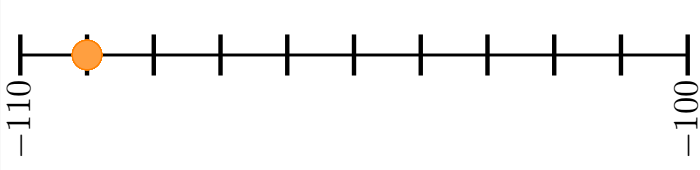
\includegraphics[width=0.8\linewidth]{../images/recta_num_-109.png} \\[-0.5em]    \qquad \fillin[$-109$][0in]

				\part 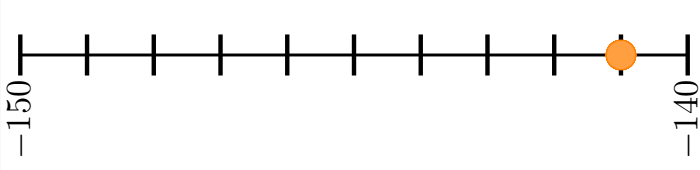
\includegraphics[width=0.8\linewidth]{../images/recta_num_-141.png} \\[-0.5em]    \qquad \fillin[$-141$][0in]

				\part 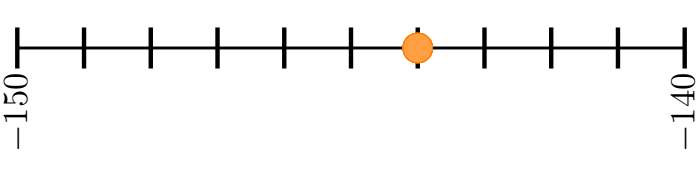
\includegraphics[width=0.8\linewidth]{../images/recta_num_-144.png}   \\[-0.5em]  \qquad \fillin[$-144$][0in]

				\part 
\includegraphics[width=0.8\linewidth]{../images/recta_num_-2.png} \\[-0.5em]  \qquad   \fillin[$-2$][0in]

				\part 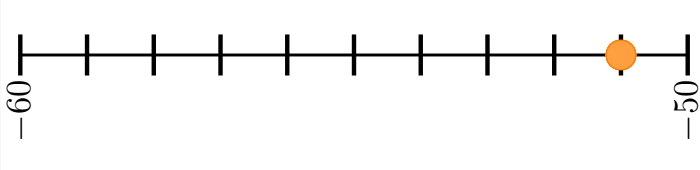
\includegraphics[width=0.8\linewidth]{../images/recta_num_-51.png}   \\[-0.5em] \qquad  \fillin[$-51$][0in]

				\columnbreak%


				\part 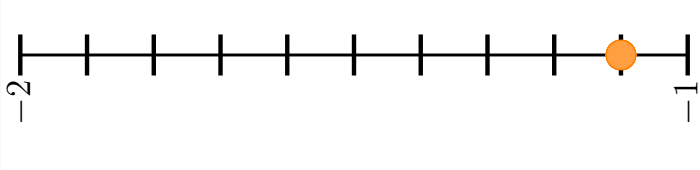
\includegraphics[width=0.8\linewidth]{../images/recta_num_-1.1.png}\\[-0.5em]   \qquad \fillin[$-1.1$][0in]

				\part 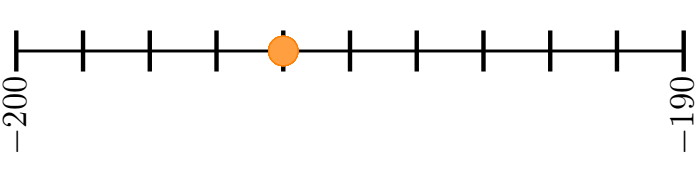
\includegraphics[width=0.8\linewidth]{../images/recta_num_-196.png}  \\[-0.5em]   \qquad \fillin[$-196$][0in]

				\part 
\includegraphics[width=0.8\linewidth]{../images/recta_num_-182.png}  \\[-0.5em]   \qquad \fillin[$-182$][0in]

				\part 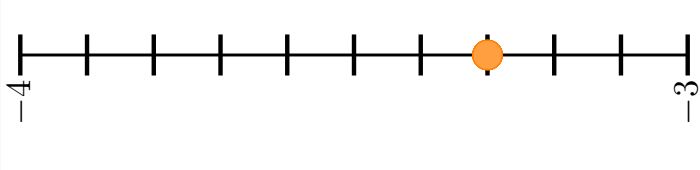
\includegraphics[width=0.8\linewidth]{../images/recta_num_-3.3.png}\\[-0.5em]   \qquad \fillin[$-3.3$][0in]

				\part 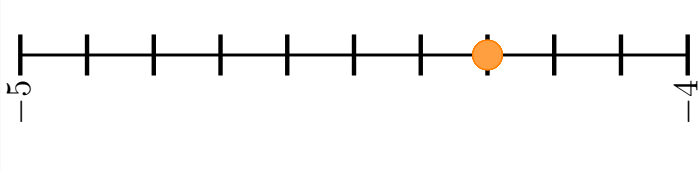
\includegraphics[width=0.8\linewidth]{../images/recta_num_-4.3.png}  \\[-0.5em]   \qquad \fillin[$-4.3$][0in]
			\end{parts}
		\end{multicols}
	}

	\subsubsection{Suma y resta con negativos}

	\questionboxed[1]{Realiza las siguientes sumas y restas con números negativos:

		\begin{multicols}{3}
			\begin{parts}
				\part $(14)+(-9)=$ \fillin[$5$][0in]

				\part $101-116=$ \fillin[$-15$][0in]

				\part $80-100=$ \fillin[$-20$][0in]

				\part $12-20=$ \fillin[$-8$][0in]

				\part $-47+35=$ \fillin[$-12$][0in]

				\part $55-99=$ \fillin[$-44$][0in]

				\part $(16)-(-20)+(39)=$ \fillin[$75$][0in]

				\part $-17-17=$ \fillin[$-34$][0in]

				\part $33-29=$ \fillin[$4$][0in]

				 \part $-223+67=$ \fillin[$-156$][0in]

				 \part $(56)-(-24)=$ \fillin[$80$][0in]

				\part $-(-25)+(-24)=$ \fillin[$1$][0in]

				\part $-235+304=$ \fillin[$69$][0in]

				\part $198-189=$ \fillin[$9$][0in]

				\part $-201.1-9.4=$ \fillin[$-210.5$][0in]

				\part $201.1-9.4=$ \fillin[$191.7$][0in]

				\part $-201.1+9.4=$ \fillin[$-191.7$][0in]

			\end{parts}
		\end{multicols}
	}


	% \addcontentsline{toc}{subsubsection}{Multiplicación y división con negativos}
	\subsubsection{Multiplicación y división con negativos}

	\questionboxed[1]{Realiza las siguientes multiplicaciones y divisiones con números negativos:

		\begin{multicols}{2}
			\begin{parts}
				\part $(-16)\divisionsymbol (-8)=$ \fillin[$-\dfrac{1}{2}$][0in]

				\part $(15)(-4)=$ \fillin[$-60$][0in]

				\part $(-80)\divisionsymbol (20)=$ \fillin[$-4$][0in]

				\part $(66)\divisionsymbol (-33)\divisionsymbol (-2)\divisionsymbol (10)=$ \fillin[$\dfrac{1}{10}$][0in]

				\part $(31)\divisionsymbol (-62)=$ \fillin[$-\dfrac{1}{2}$][0in]

				\part $(-18)(-25)=$ \fillin[$450$][0in]

				\part $(-4)\divisionsymbol (5)\divisionsymbol (-1)=$ \fillin[$20$][0in]

				\part $(-7)(20)=$ \fillin[$-140$][0in]

				\part $(60)\divisionsymbol (-2)\divisionsymbol (-10)=$ \fillin[$-3$][0in]

				\part $(-11)\divisionsymbol (9)=$ \fillin[$-\dfrac{11}{9}$][0in]

				\part $(-11)(-6)(2)(-3)=$ \fillin[$-396$][0in]

				\part $(25) \divisionsymbol (-3) \divisionsymbol (-5) \divisionsymbol(-10)=$ \fillin[$-\dfrac{1}{6}$][0in]

				\part $(-6)(-6)(-6)=$ \fillin[$-216$][0in]

				\part $(-220)\divisionsymbol (0.2)=$ \fillin[$-1100$][0in]
			\end{parts}
		\end{multicols}
	}


	% \addcontentsline{toc}{subsubsection}{Potencias con números negativos}
	\subsubsection{Potencias con números negativos}

	\questionboxed[1]{Realiza las siguientes potencias de números negativos:

		\begin{multicols}{3}
			\begin{parts}
				\part $-2^{9}=$ \fillin[$-512$][0in] \\[-0.5em]
				\part $-1^{80}=$ \fillin[$-1$][0in] \\[-0.5em]
				\part $(-5)^3=$ \fillin[$-125$][0in] \\[-0.5em]
				\part $-5^4=$ \fillin[$-625$][0in] \\[-0.5em]
				\part $(-1)^{75}=$ \fillin[$-1$][0in] \\[-0.5em]
				\part $(-3)^4=$ \fillin[$81$][0in] \\[-0.5em]
				\part $(-10)^3=$ \fillin[$-1000$][0in] \\[-0.5em]
				\part $-10^4=$ \fillin[$-10000$][0in] \\[-0.5em]
				\part $-(-2)^4=$ \fillin[$-16$][0in] \\[-0.5em]
				\part $-(-6)^3=$ \fillin[$216$][0in] \\[-0.5em]
				\part $(-6)^3=$ \fillin[$-216$][0in] \\[-0.5em]
				\part $-6^3=$ \fillin[$-216$][0in] \\[-0.5em]
				\part $(-2)^{10}=$ \fillin[$1024$][0in] \\[-0.5em]
				\part $-(-2)^9=$ \fillin[$512$][0in] \\[-0.5em]
				\part $(-2)^9=$ \fillin[$-512$][0in] \\[-0.5em]
			\end{parts}
		\end{multicols}
	}

	% \addcontentsline{toc}{subsection}{Exponentes y notación científica}
	\subsection{Exponentes y notación científica}

	\subsubsection{Suma de exponentes}

	\questionboxed[2]{Realiza las siguientes operaciones con exponentes:

		\begin{multicols}{3}
			\begin{parts}
				\part $(-5a^4)(-3a^2)=$ \fillin[$15a^6$][0in]

				% \begin{solutionbox}{1cm}
				% 	$(-5a^4)(-3a^2) = 15a^6$
				% \end{solutionbox}


				\part $(5x^3)(-x^{11})=$ \fillin[$-5x^{14}$][0in]

					% \begin{solutionbox}{1cm}
				% 	$(5x^3)(-x^{11})= -5x^{14}$
				% \end{solutionbox}

				\part $x^4x^{12}x^7=$ \fillin[$x^{23}$][0in]


				% \begin{solutionbox}{1cm}
				% 	$x^4x^{12}x^7= x^{23}$
				% \end{solutionbox}


				\part $(-2a^3)(-a)=$ \fillin[$-2a^4$][0in]

				% \begin{solutionbox}{1cm}
				% 	$(-2a^3)(-a)= -2a^4$
				% \end{solutionbox}


				\part $(5y^5)(7y^4)=$  \fillin[$35y^9$][0in]

				% \begin{solutionbox}{1cm}
				% 	$(5y^5)(7y^4)=35y^9$
				% \end{solutionbox}


				\part $(-3a^4)(8a^2)=$ \fillin[$-24a^6$][0in]

				% \begin{solutionbox}{1cm}
					% $(-3a^4)(8a^2) = -24a^6$
				% \end{solutionbox}


				\part $4x^2\cdot x^5\cdot 5x^8=$ \fillin[$20x^{15}$][0in]

				% \begin{solutionbox}{1cm}
				% 	$4x^2\cdot x^5\cdot 5x^8 = 20x^{15}$
				% \end{solutionbox}


				\part $x^2y^3z^4 \cdot x^5z^4=$ \fillin[$x^7y^3z^8$][0in]

				% \begin{solutionbox}{1cm}
				% 	$x^2y^3z^4 \cdot x^5z^4 = x^7y^3z^8$
				% \end{solutionbox}


				\part $7x^2\cdot 3x^4 \cdot 6x^2=$  \fillin[$126x^8$][0in]

				% \begin{solutionbox}{1cm}
				% 	$7x^2\cdot 3x^4 \cdot 6x^2 = 126x^8$
				% \end{solutionbox}

			\end{parts}
		\end{multicols}
	}

	\subsubsection{Resta de exponentes}

	\questionboxed[3]{Realiza las siguientes operaciones con exponentes:

		\begin{multicols}{3}
			\begin{parts}
				\part $\dfrac{18x^{15}}{6x^{12}}=$ \fillin[$3x^3$][0in]

				% \begin{solutionbox}{1.5cm}
				% 	$\dfrac{18x^{15}}{6x^{12}}=3x^3$
				% \end{solutionbox}

				\part $\dfrac{6x^{7}}{2x^{2}}=$ \fillin[$3x^5$][0in]

				% \begin{solutionbox}{1.5cm}
				% 	$\dfrac{6x^{7}}{2x^{2}}=3x^5$
				% \end{solutionbox}

				\part $\dfrac{a^3b^{9}c^5}{a^2b^{5}c^4}=$ \fillin[$ab^4c$][0in]

				% \begin{solutionbox}{1.5cm}
				% 	$\dfrac{a^3b^{9}c^5}{a^2b^{5}c^4}=ab^4c$
				% \end{solutionbox}

				\part $\dfrac{x^{13}y^{18}z^{4}}{x^{11}y^{9}z^{4}}=$ \fillin[$x^2y^9$][0in]

				% \begin{solutionbox}{1.5cm}
				% 	$\dfrac{x^{13}y^{18}z^{4}}{x^{11}y^{9}z^{4}} = x^2y^9$
				% \end{solutionbox}

				\part $\dfrac{21x^{23}}{7x^{11}}=$ \fillin[$3x^{12}$][0in]

				% \begin{solutionbox}{1.5cm}
				% 	$\dfrac{21x^{23}}{7x^{11}}=3x^{12}$
				% \end{solutionbox}

				\part $\dfrac{25x^{8}}{5x^{3}}=$ \fillin[$5x^5$][0in]

				% \begin{solutionbox}{1.5cm}
				% 	 $\dfrac{25x^{8}}{5x^{3}}=5x^5$
				% \end{solutionbox}

				\part $\dfrac{x^{3}y^{12}z^{13}}{x^{3}y^{12}z^{13}}=$ \fillin[$1$][0in]

				% \begin{solutionbox}{1.5cm}
				% 	$\dfrac{x^{3}y^{12}z^{13}}{x^{3}y^{12}z^{13}} = 1$
				% \end{solutionbox}

				\part $\dfrac{81a^5b^{12}c^9}{9a^3b^{7}c^5}=$ \fillin[$9a^2b^5c^4$][0in]

				% \begin{solutionbox}{1.5cm}
				% 	$\dfrac{81a^5b^{12}c^9}{9a^3b^{7}c^5} = 9a^2b^5c^4$
				% \end{solutionbox}

				\part $\dfrac{5x^{8}}{25x^{3}}=$ \fillin[$\dfrac{x^5}{5}$][0in]

				% \begin{solutionbox}{1.5cm}
				% 	$\dfrac{5x^{8}}{25x^{3}}=\dfrac{x^5}{5}$
				% \end{solutionbox}
			\end{parts}
		\end{multicols}
	}	

	\subsubsection{Multiplicación de exponentes}

	\questionboxed[1]{Realiza las siguientes operaciones con exponentes:

	\begin{multicols}{3}
		\begin{parts}
			\part $(a^3b^2c^4)^3=$ \fillin[$a^9b^6c^{12}$][0in]

			% \begin{solutionbox}{1cm}
			% 	$(a^3b^2c^4)^3 = a^9b^6c^{12}$
			% \end{solutionbox}
			\part $(x^9y^5z^2)^5=$ \fillin[$x^{45}y^{25}z^{10}$][0in]

			\part $(a^4b^5)^4=$ \fillin[$a^{16}b^{20}$][0in]

			\part $\left(x^9 y^5\right)^{11}=$  \fillin[$x^{99}y^{55}$][0in]

			\part $\left(x^4 y^5\right)^6=$  \fillin[$x^{24}y^{30}$][0in]

			% \begin{solutionbox}{1cm}
			% 	$\left(x^4 y^5\right)^6 = x^{24}y^{30}$
			% \end{solutionbox}

			\part $(x^7y^8z^4w^5)^6=$ \fillin[$x^{42}y^{48}z^{24}w^{30}$][0in]

			\part $(a^3b^7c^5d^4)^4=$ \fillin[$a^{12}b^{28}c^{20}d^{16}$][0in]

			\part $\left(a^3 b^5 c^{11} \right)^7=$  \fillin[$a^{21}b^{35}c^{77}$][0in]

			% \begin{solutionbox}{1cm}
			% 	$\left(a^3 b^5 c^{11} \right)^7 = a^{21}b^{35}c^{77}$
			% \end{solutionbox}

			\part $(a^4b^4c^5d^{11})^5=$ \fillin[$a^{20}b^{20}c^{25}d^{55}$][0in]

		\end{parts}
	\end{multicols}
}	

	\subsubsection{Notación científica}

	\questionboxed[1]{Escribe en notación científica los siguientes números:

		\begin{multicols}{3}
			\begin{parts}
				\part $55000=$ \fillin[$5.5 \times 10^4$][0in]

				\part $0.00000000024=$ \fillin[$2.4 \times 10^{-10}$][0in]

				\part $101=$ \fillin[$1.01 \times 10^2$][0in]

				\part $750000000000=$ \fillin[$7.5 \times 10^{11}$][0in]

				\part $0.000000015=$ \fillin[$1.5 \times 10^{-7}$][0in]

				\part $900000000000=$ \fillin[$9 \times 10^{11}$][0in]
				 
				\part $80000000=$ \fillin[$8 \times 10^7$][0in]

				\part $0.003=$ \fillin[$3 \times 10^{-3}$][0in]

				\part $0.0000204=$ \fillin[$2.04 \times 10^{-5}$][0in]

				\part $0.000000099=$ \fillin[$9.9 \times 10^{-9}$][0in]

				\part $606000000=$ \fillin[$6.06 \times 10^{8}$][0in]

				\part $10210000000=$ \fillin[$1.021 \times 10^{10}$][0in]

			\end{parts}
		\end{multicols}
	}

	\questionboxed[2]{Escribe en notación decimal los siguientes números:

		\begin{multicols}{4}
			\begin{parts}
				\part $1.2 \times 10^3=$ \fillin[$1200$][0in]

				\part $2.3 \times 10^2=$ \fillin[$230$][0in]

				\part $4 \times 10^{-3}=$ \fillin[$0.004$][0in]

				\part $7 \times 10^{-6}=$ \fillin[$0.000007$][0in]

				\part $2 \times 10^5=$ \fillin[$200000$][0in]

				\part $-3 \times 10^{-2}=$ \fillin[$-0.03$][0in]

				\part $9 \times 10^{0}=$ \fillin[$9$][0in]

				\part $6.3 \times 10^{-3}=$ \fillin[$0.0063$][0in]

				\part $1.2 \times 10^{-1}=$ \fillin[$0.12$][0in]

				\part $80.3 \times 10^{-2}=$ \fillin[$0.803$][0in]

				\part $3 \times 10^{-3}=$ \fillin[$0.003$][0in]

				\part $3 \times 10^{8}=$ \fillin[$300000000$][0in]

			\end{parts}
		\end{multicols}
	}

	\subsection{Plano cartesiano y la recta}

	\subsubsection{Ubicación en el plano cartesiano}

	\questionboxed[3]{Escribe las coordenadas de los puntos indicados en el plano cartesiano de cada uno de los siguientes incisos.

		\begin{multicols}{2}
			\begin{parts}
				\part Coordenadas del punto A: \fillin[$(1,5)$][0in]

				\part Coordenadas del punto B: \fillin[$(-3,6)$][0in]

				\part Coordenadas del punto C: \fillin[$(5,-3)$][0in]

				\part Coordenadas del punto D: \fillin[$(-5,0)$][0in]

				\part Coordenadas del punto E: \fillin[$(0,-7)$][0in]

				\part El punto C está en el cuadrante: \fillin[IV][0in]

				\part El punto B está en el cuadrante: \fillin[II][0in]

				\part El punto A está en el cuadrante: \fillin[I][0in]
			\end{parts}
			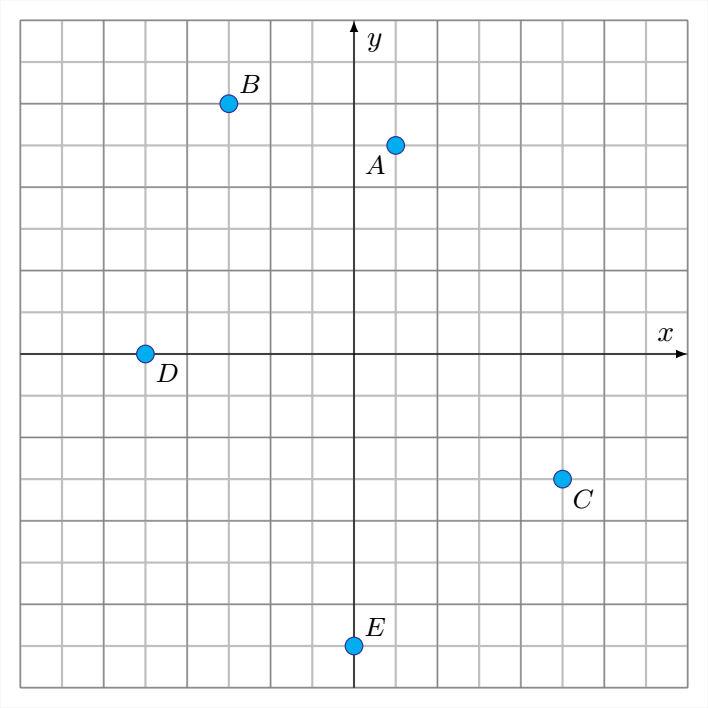
\includegraphics[width=0.75\linewidth]{../images/plano_cart02.png}
		\end{multicols}
	}


	\questionboxed[3]{Escribe las coordenadas de los puntos indicados en el plano cartesiano de cada uno de los siguientes incisos.

		\begin{multicols}{2}
			\begin{parts}
				\part Coordenadas del punto A: \fillin[$(1,4)$][0in]

				\part Coordenadas del punto B: \fillin[$(3,3)$][0in]

				\part Coordenadas del punto C: \fillin[$(-3,1)$][0in]

				\part Coordenadas del punto D: \fillin[$(3,0)$][0in]

				\part Coordenadas del punto E: \fillin[$(0,-1)$][0in]

				\part El punto A está en el cuadrante: \fillin[I][0in]

				\part El punto B está en el cuadrante: \fillin[I][0in]

				\part El punto C está en el cuadrante: \fillin[II][0in]
			\end{parts}
			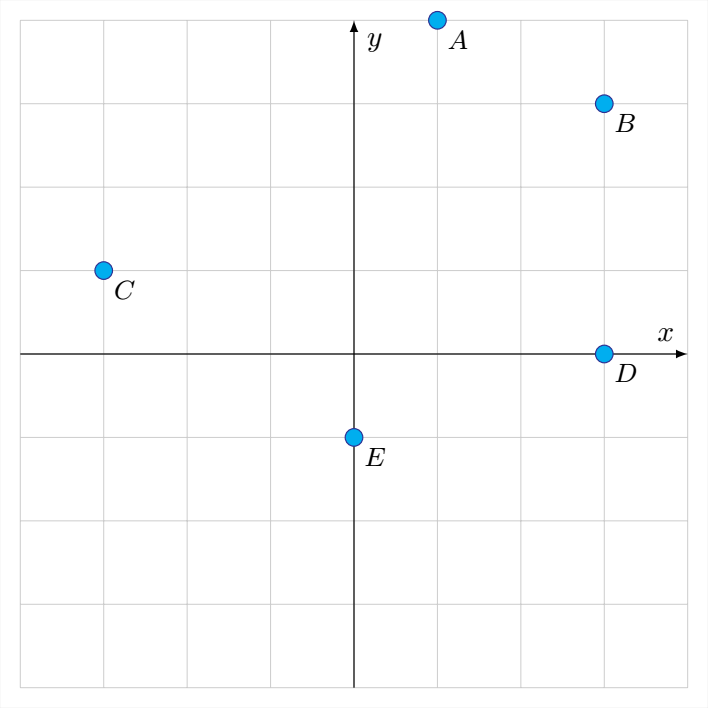
\includegraphics[width=0.75\linewidth]{../images/plano_cart03.png}
		\end{multicols}
	}

	\questionboxed[3]{Escribe las coordenadas de los puntos indicados en el plano cartesiano de cada uno de los siguientes incisos.

		\begin{multicols}{2}
			\begin{parts}
				\part Coordenadas del punto A: \fillin[$(0,1)$][0in]

				\part Coordenadas del punto B: \fillin[$(3,-4)$][0in]

				\part Coordenadas del punto C: \fillin[$(2,-3)$][0in]

				\part Coordenadas del punto D: \fillin[$(0,0)$][0in]

				\part Coordenadas del punto E: \fillin[$(0,-3)$][0in]

				\part El punto B está en el cuadrante: \fillin[IV][0in]

				\part El punto C está en el cuadrante: \fillin[IV][0in]
			\end{parts}
			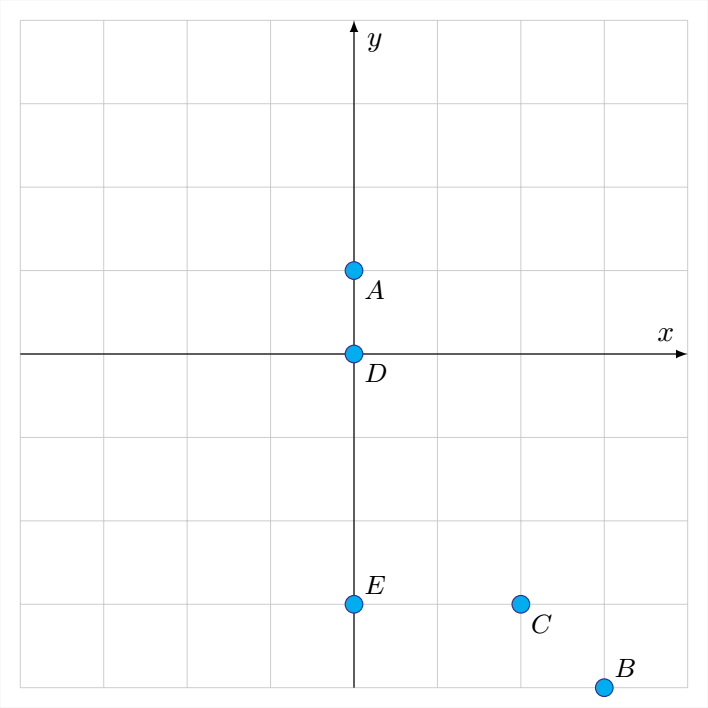
\includegraphics[width=0.75\linewidth]{../images/plano_cart01.png}
		\end{multicols}
	}

	\subsubsection{Pendiente de una recta}

	\questionboxed[5]{Selecciona la opcion que corresponde a la pendiente de la recta en cada uno de los siguientes incisos:

		\begin{multicols}{2}
			\begin{parts}
				\part
				\begin{minipage}{0.6\linewidth}
					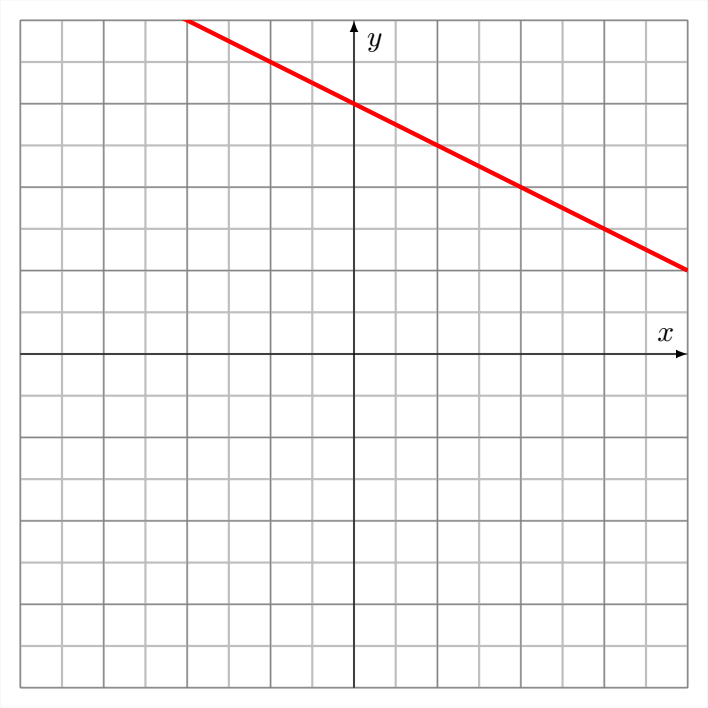
\includegraphics[width=0.8\linewidth]{../images/plano_cart_rect_-1|2x+4.png}
				\end{minipage}%
				\begin{minipage}{0.5\linewidth}
					\begin{choices}
						\choice Positiva
						\CorrectChoice Negativa
						\choice Cero
						\choice Indefinida
					\end{choices}
				\end{minipage}

				\part
				\begin{minipage}{0.6\linewidth}
					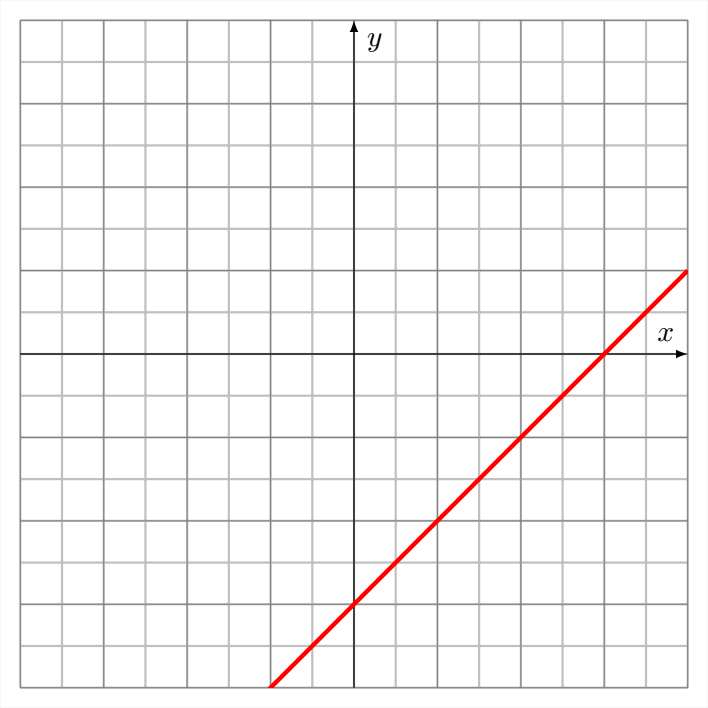
\includegraphics[width=0.8\linewidth]{../images/plano_cart_rect_x-6.png}
				\end{minipage}%
				\begin{minipage}{0.5\linewidth}
					\begin{choices}
						\CorrectChoice Positiva
						\choice Negativa
						\choice Cero
						\choice Indefinida
					\end{choices}
				\end{minipage}

				\part
				\begin{minipage}{0.6\linewidth}
					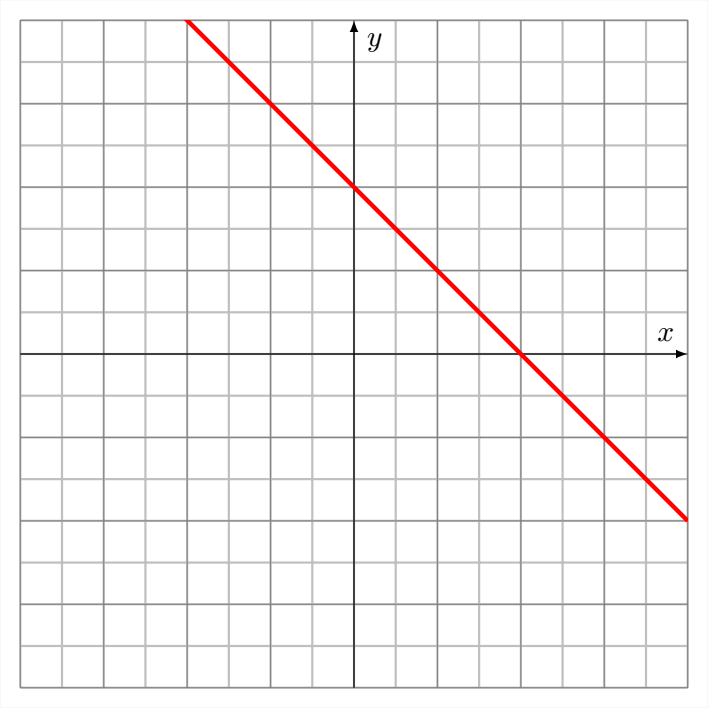
\includegraphics[width=0.8\linewidth]{../images/plano_cart_rect_-x+4.png}
				\end{minipage}%
				\begin{minipage}{0.5\linewidth}
					\begin{choices}
						\choice Positiva
						\CorrectChoice Negativa
						\choice Cero
						\choice Indefinida
					\end{choices}
				\end{minipage}
				
				
				\part
				\begin{minipage}{0.6\linewidth}
					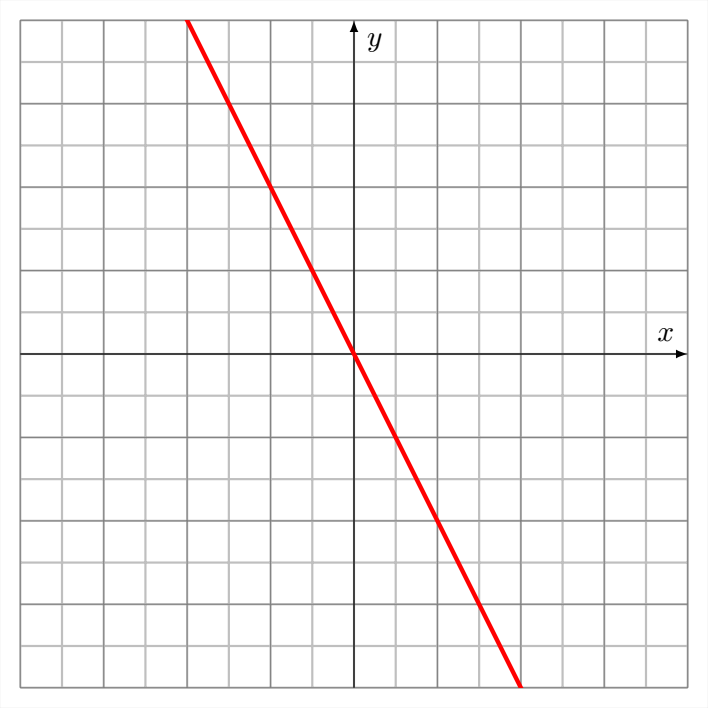
\includegraphics[width=0.8\linewidth]{../images/plano_cart_rect_-2x.png}
				\end{minipage}%
				\begin{minipage}{0.5\linewidth}
					\begin{choices}
						\choice Positiva
						\CorrectChoice Negativa
						\choice Cero
						\choice Indefinida
					\end{choices}
				\end{minipage}

				\part
				\begin{minipage}{0.6\linewidth}
					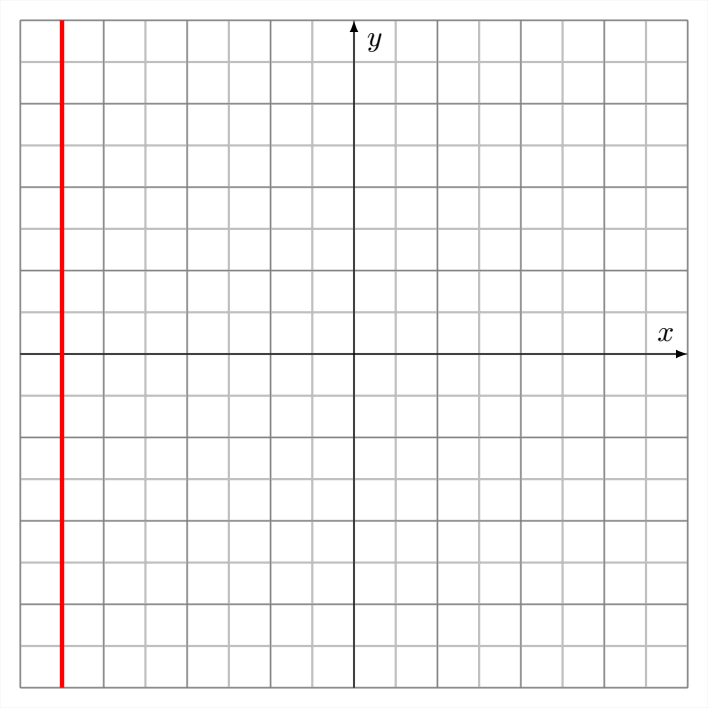
\includegraphics[width=0.8\linewidth]{../images/plano_cart_rect_inf.png}
				\end{minipage}%
				\begin{minipage}{0.5\linewidth}
					\begin{choices}
						\choice Positiva
						\choice Negativa
						\choice Cero
						\CorrectChoice Indefinida
					\end{choices}
				\end{minipage}

				\part
				\begin{minipage}{0.6\linewidth}
					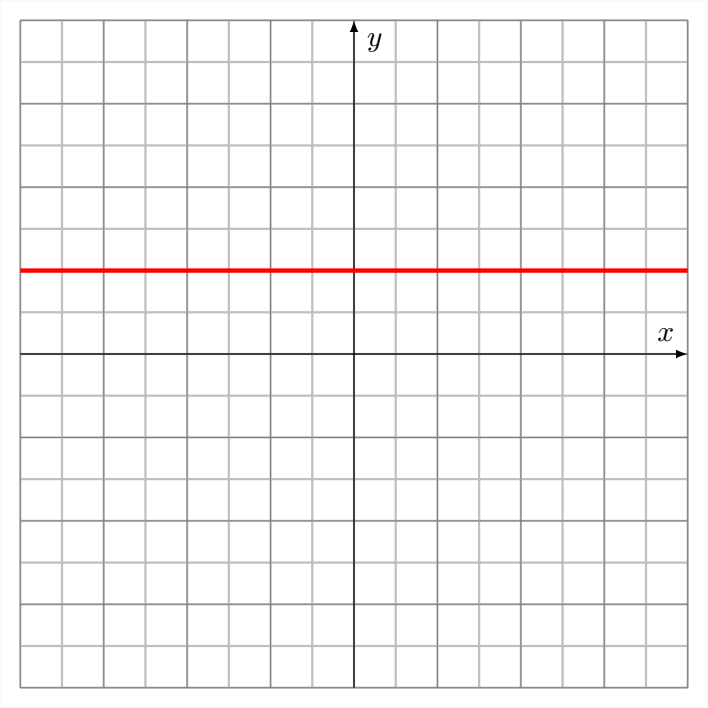
\includegraphics[width=0.8\linewidth]{../images/plano_cart_rect_0.png}
				\end{minipage}%
				\begin{minipage}{0.5\linewidth}
					\begin{choices}
						\choice Positiva
						\choice Negativa
						\CorrectChoice Cero
						\choice Indefinida
					\end{choices}
				\end{minipage}
			\end{parts}
		\end{multicols}
	}


	% \addcontentsline{toc}{subsubsection}{Pendiente y ordenada}
	\subsubsection{Pendiente y ordenada}

	\questionboxed[1]{Identifica la pendiente y ordenada de las siguientes rectas:

		\begin{multicols}{3}
			\begin{parts}
				\part $y=-2x$ \\[1em]
				Pendiente = \fillin[$-2$][0in]\\[0.5em]
				Ordenada = \fillin[$0$][0in]

				\part $y=-\dfrac{2}{3}x-5$ \\[1em]
				Pendiente = \fillin[$-\dfrac{2}{3}$][0in]\\[0.5em]
				Ordenada = \fillin[$-5$][0in]

				\part $y=3x+2$ \\[1em]
				Pendiente = \fillin[$3$][0in]\\[0.5em]
				Ordenada = \fillin[$2$][0in]

				\part $y=\dfrac{1}{2}x-3$ \\[1em]
				Pendiente = \fillin[$\dfrac{1}{2}$][0in]\\[0.5em]
				Ordenada = \fillin[$-3$][0in]

				\part $y=-\dfrac{1}{2}x+3$ \\[1em]
				Pendiente = \fillin[$-\dfrac{1}{2}$][0in]\\[0.5em]
				Ordenada = \fillin[$3$][0in]

				\part $y=-3x+3$ \\[1em]
				Pendiente = \fillin[$-3$][0in]\\[0.5em]
				Ordenada = \fillin[$3$][0in]
			\end{parts}
		\end{multicols}
	}


	% \addcontentsline{toc}{subsubsection}{Ecuación de una recta}
	\subsubsection{Ecuación de una recta}

	\questionboxed[1]{Escribe la ecuación de cada una de las rectas en los siguientes planos cartesianos:

		\begin{multicols}{2}
			\begin{parts}
				\part
				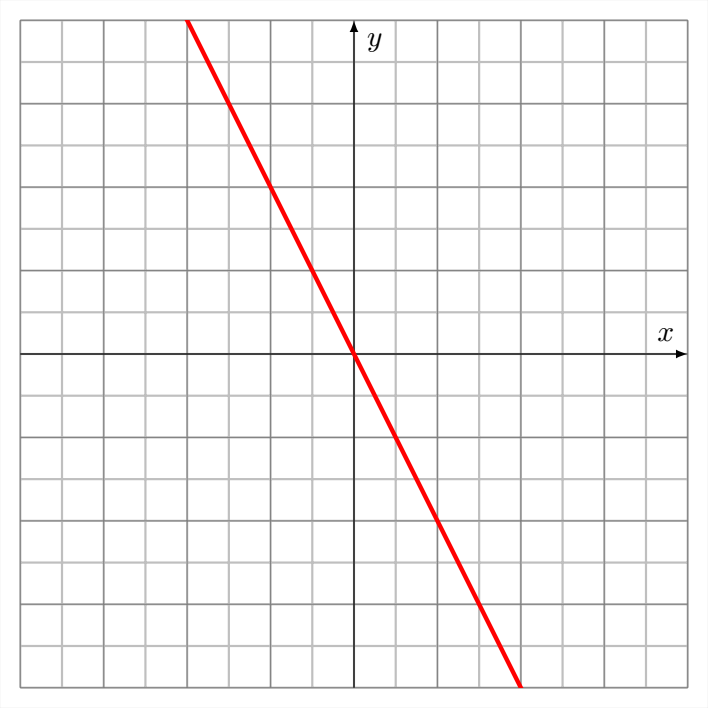
\includegraphics[width=.6\linewidth]{../images/plano_cart_rect_-2x.png}\\
				\fillin[$y=-2x$][2in]

				\part
				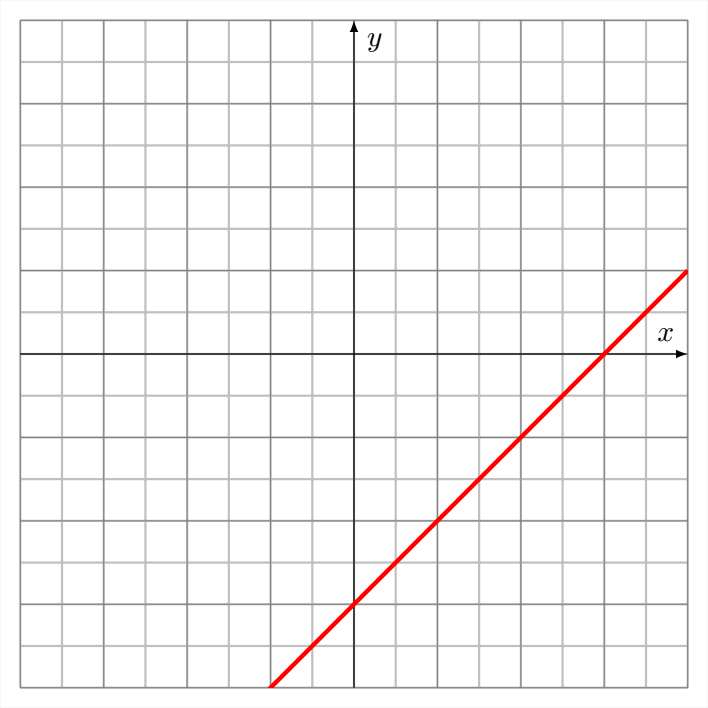
\includegraphics[width=.6\linewidth]{../images/plano_cart_rect_x-6.png}\\
				\fillin[$y=x-6$][2in]
			\end{parts}
		\end{multicols}
	}

	% \addcontentsline{toc}{subsection}{Porcentajes}
	\subsection{Porcentajes}

	% \addcontentsline{toc}{subsubsection}{Porcentajes a decimal}
	\subsubsection{Porcentajes a decimal}

	\questionboxed[1]{Escribe el número decimal que representa cada porcentaje:

		\begin{multicols}{2}
			\begin{parts}
				\part Convierte 401\% a un número decimal. \fillin[$4.01$][0in]
				\part Convierte 100\% a un número decimal. \fillin[$1$][0in]
				\part Convierte 10\% a un número decimal. \fillin[$0.1$][0in]
				\part Convierte 6\% a un número decimal. \fillin[$0.06$][0in]
				\part Convierte 0.5\% a un número decimal. \fillin[$0.005$][0in]
				\part Convierte 150\% a un número decimal. \fillin[$1.5$][0in]
				\part Convierte 33\% a un número decimal. \fillin[$0.33$][0in]
				\part Convierte 20.9\% a un número decimal. \fillin[$0.209$][0in]
				\part Convierte 3.2\% a un número decimal. \fillin[$0.032$][0in]
				\part Convierte 37.5\% a un número decimal. \fillin[$0.375$][0in]
			\end{parts}
		\end{multicols}
	}


	% \addcontentsline{toc}{subsubsection}{Decimal a porcentaje}
	\subsubsection{Decimal a porcentaje}

	\questionboxed[1]{Escribe el porcentaje que representa cada número decimal:

		\begin{multicols}{2}
			\begin{parts}
				\part Expresa 1.44 como un porcentaje. \fillin[$144\%$][0in]
				\part Expresa 1 como un porcentaje. \fillin[$100\%$][0in]
				\part Expresa 0.1 como un porcentaje. \fillin[$10\%$][0in]
				\part Expresa 2.5 como un porcentaje. \fillin[$250\%$][0in]
				\part Expresa 0.001 como un porcentaje. \fillin[$0.1\%$][0in]
				\part Expresa 0.9 como un porcentaje. \fillin[$90\%$][0in]
				\part Expresa 0.05 como un porcentaje. \fillin[$5\%$][0in]
				\part Expresa 0.33 como un porcentaje. \fillin[$33\%$][0in]
				\part Expresa 0.092 como un porcentaje. \fillin[$9.2\%$][0in]
				\part Expresa 0.209 como un porcentaje. \fillin[$20.9\%$][0in]
			\end{parts}
		\end{multicols}
	}


	% \addcontentsline{toc}{subsubsection}{Porcentaje de cantidades}
	\subsubsection{Porcentaje de cantidades}

	\questionboxed[1]{Calcula los porcentajes de cada una de las siguientes cantidades:

		\begin{multicols}{2}
			\begin{parts}
				\part ¿Cuál es el 225\% de 600?
				
				\begin{solutionbox}{1.2cm}
					\[\dfrac{600\times 225\%}{100\%}=1350\]
				\end{solutionbox}

				\part Si se sabe que 30 es el 6\% de cierta cantidad, ¿cuál es esta cantidad?
				
				\begin{solutionbox}{1.2cm}
					\[\dfrac{30\times 100\%}{6\%}=500\]
				\end{solutionbox}

				\part ¿Cuál es el 23\% de 59?
				
				\begin{solutionbox}{1.2cm}
					\[\dfrac{59\times 23\%}{100\%}=13.57\]
				\end{solutionbox}

				\part Si se sabe que 40 es el 250\% de cierta cantidad, ¿cuál es esta cantidad?
				
				\begin{solutionbox}{1.2cm}
					\[\dfrac{40\times 100\%}{250\%}=16\]
				\end{solutionbox}
			\end{parts}
		\end{multicols}
	}

	\subsubsection{Resolución de problemas}

	\questionboxed[2]{Resuelve los siguientes problemas:

		\begin{parts}
			\part El costo de una camisa es de \$800 pesos, si se les hace un descuento del 20\%, ¿cuánto pagaré en total por la camisa?
			
			\begin{solutionbox}{1.5cm}
				\[\$800\times 20\%=\$160\]
				\[\$800-\$160=\$640\]
			\end{solutionbox}

			\part El 24\% de los habitantes de un pueblo tienen menos de 30 años. ¿Cuántos habitantes tiene el pueblo si hay 120 jóvenes menores de 30 años?
			
			\begin{solutionbox}{1.2cm}
				\[\dfrac{120\times 100\%}{24\%}=500\]
			\end{solutionbox}
		\end{parts}
	}

	\section{Unidad 2}

\subsection{Círculo}
	\subsubsection{Resolución de problemas}

	\questionboxed[1]{Resuelve los siguientes problemas:

		\begin{multicols}{2}
			\begin{parts}
				\part Una casa tiene una alberca circular de 6 metros de diámetro. Calcula el área de la alberca.
				% \fillin[$28.26$ m$^2$][0in]

				\begin{solutionbox}{1cm}
					$A=\pi r^2 = \pi (3)^2 = 28.26$ m$^2$
				\end{solutionbox}


				\part El radio de una rueda es de 32 centímetros, ¿cuántos centímetros habrá recorrido esa rueda después de haber dado 22 vueltas?
				%  \fillin[$70737.92$ cm][0in]

				\begin{solutionbox}{1.2cm}
					$C=2\pi r = 2\pi (32) = 201.06$ cm\\
					$22(201.06) = 70737.92$ cm
				\end{solutionbox}

				\columnbreak%


				\part Calcula el área de un parque que tiene un radio de 170 metros.
				%\fillin[$90746$ m][0in]

				\begin{solutionbox}{1cm}
					$A=\pi r^2 = \pi (170)^2 = 90746$ m$^2$
				\end{solutionbox}

				\part Daniel tiene un terreno circular con un radio de 6 metros al cual le desea poner una barda en su periferia, si el precio por metro de barda es de 124 pesos. ¿Cuánto pagará en total por poner la barda?
				%\fillin[$\$4,672.32$ pesos][0in]

				\begin{solutionbox}{1.2cm}
					$P=2\pi r = 2\pi (6) = 37.68$ m\\
					$37.68(124) = \$4672.32$ pesos
				\end{solutionbox}
			\end{parts}
		\end{multicols}
	}

	\subsubsection{Radio, Diámetro, Perímetro y Área de un círculo}

	% \questionboxed[3]{Encuentra el \textbf{perímetro} y el \textbf{área} de los siguientes círculos:

	% 	\begin{multicols}{3}
	% 		\begin{parts}
	% 			% \part 
\includegraphics[width=0.85\linewidth]{mex_0001.png}\\
	% 			% Perímetro: \fillin[][0.3in] \quad Área: \fillin[][0.3in]
	% 			\part 
\includegraphics[width=0.85\linewidth]{mex_0002.png}\\

	% 			Perímetro: \\
	% 			\fillin[$P=2\pi r=2(3.14)51=320.28$][0in] \\
	% 			Área: \\
	% 			\fillin[$A=\pi r^2=3.14(51)^2=8167.14$][0in] 

	% 			% \part 
\includegraphics[width=0.85\linewidth]{mex_0003.png}\\
	% 			% Perímetro: \fillin[][0.3in] \quad Área: \fillin[][0.3in]
	% 			% \part 
\includegraphics[width=0.85\linewidth]{mex_0004.png}\\
	% 			% Perímetro: \fillin[][0.3in] \quad Área: \fillin[][0.3in]
	% 			\part 
\includegraphics[width=0.85\linewidth]{mex_0005.png}\\

	% 			Perímetro: \\
	% 			\fillin[$P=\pi d=(3.14)14.2=44.58$][0in] \\
	% 			Área: \\
	% 			\fillin[$A=\pi \left(\frac{d}{2}\right)^2=3.14\left(\frac{14.2}{2}\right)^2=158.28$][0in] 

	% 			\part 
\includegraphics[width=0.85\linewidth]{mex_0009.png}\\

	% 			Perímetro: \\
	% 			\fillin[$P=\pi d=(3.14)49.1=154.17$][0in] \\
	% 			Área: \\
	% 			\fillin[$A=\pi \left(\frac{d}{2}\right)^2=3.14\left(\frac{49.1}{2}\right)^2=1892.48$][0in] 
	% 		\end{parts}
	% 	\end{multicols}
	% }	

	\questionboxed[3]{Encuentra el \textbf{perímetro} y el \textbf{área} de los siguientes círculos:

		\begin{multicols}{3}
			\begin{parts}
				\part 
\includegraphics[width=0.85\linewidth]{mex_0006.png}\\

				Perímetro: \\
				\fillin[$P=2\pi r=2(3.14)27=169.56$][0in] \\
				Área: \\
				\fillin[$A=\pi r^2=3.14(27)^2=2289.06$][0in] 

				% \part 
\includegraphics[width=0.85\linewidth]{mex_0007.png}\\
				% Perímetro: \fillin[][0.3in] \quad Área: \fillin[][0.3in]
				\part 
\includegraphics[width=0.85\linewidth]{mex_0008.png}\\

				Perímetro: \\
				\fillin[$P=2\pi r=2(3.14)21.82=137.02$][0in] \\
				Área: \\
				\fillin[$A=\pi r^2=3.14(21.82)^2=1494.99$][0in] 

				% \part 
\includegraphics[width=0.85\linewidth]{mex_0010.png}\\
				% Perímetro: \fillin[][0.3in] \quad Área: \fillin[][0.3in]
				\part 
\includegraphics[width=0.85\linewidth]{mex_0011.png}\\

				Perímetro: \\
				\fillin[$P=2\pi r=2(3.14)10=62.8$][0in] \\
				Área: \\
				\fillin[$A=\pi r^2=3.14(10)^2=314$][0in] 

				% \part 
\includegraphics[width=0.85\linewidth]{mex_0012.png}\\
				% Perímetro: \fillin[][0.3in] \quad Área: \fillin[][0.3in]
			\end{parts}
		\end{multicols}
	}

	\newpage
	\subsection{Polígonos y circunferencias}
	\subsubsection{Ángulos interiores}

	\questionboxed[1]{Responde a las siguientes preguntas:

		\begin{multicols}{2}
			\begin{parts}
				% \part ¿Cuánto mide el ángulo interior de un hexágono regular? \fillin[$120$][0in]

				% \begin{solutionbox}{2cm}
				% \end{solutionbox}

				% \part ¿Cuánto mide el ángulo interior de un pentadecágono regular? \fillin[$156$][0in]

				% \begin{solutionbox}{2cm}
				% \end{solutionbox}

				\part La suma de los ángulos interiores de un polígono de 8 lados es:% \fillin[$1080$][0in]

				\begin{solutionbox}{1cm}
					\[\Sigma A_I=(n-2)(180^{\circ})=6(180^{\circ})=1080\]
				\end{solutionbox}

				\part ¿Cuánto mide el ángulo interior de un dodecágono regular?% \fillin[$150$][0in]

				\begin{solutionbox}{1cm}
					$A_I=\frac{(n-2)(180^{\circ})}{n} =\frac{(12-2)(180^{\circ})}{12} =150$
				\end{solutionbox}

				\part La suma de los ángulos interiores de un polígono de 11 lados es: %\fillin[$1620$][0in]

				\begin{solutionbox}{1cm}
					\[ \Sigma A_I=(n-2)(180^{\circ})=9(180^{\circ})=1620\]
				\end{solutionbox}

				\part ¿Cuánto mide el ángulo interior de un icoságono regular? %\fillin[$162$][0in]

				\begin{solutionbox}{1cm}
					$A_I=\frac{(n-2)(180^{\circ})}{n}= \frac{(20-2)(180^{\circ})}{20}=162$
				\end{solutionbox}
			\end{parts}
		\end{multicols}
	}

	\subsubsection{Ángulos centrales y exteriores}

	\questionboxed[1]{Responde a las siguientes preguntas:

		\begin{multicols}{2}
			\begin{parts}
				\part ¿Cuánto mide el ángulo central de un polígono de 9 lados? %\fillin[$40$][0in]

				\begin{solutionbox}{1.2cm}
					\[A_C=\frac{360^{\circ}}{n}=\frac{360^{\circ}}{9}=40^{\circ}\]
				\end{solutionbox}

				\part ¿Cuánto mide el ángulo exterior de un polígono de 10 lados? %\fillin[$36$][0in]

				\begin{solutionbox}{1.2cm}
					\[A_E=\frac{360^{\circ}}{n}=\frac{360^{\circ}}{10}=36^{\circ}\]
				\end{solutionbox}

				% \part ¿Cuánto mide el ángulo central de un polígono de 15 lados? \fillin[$24$][0in]

				% \begin{solutionbox}{2cm}
				% \end{solutionbox}

				% \part ¿Cuánto mide el ángulo central de un polígono de 12 lados? \fillin[$30$][0in]

				% \begin{solutionbox}{2cm}
				% \end{solutionbox}

				\part ¿Cuánto mide el ángulo exterior de un polígono de 6 lados? %\fillin[$60$][0in]

				\begin{solutionbox}{1.2cm}
					\[A_E=\frac{360^{\circ}}{n}=\frac{360^{\circ}}{6}=60^{\circ}\]
				\end{solutionbox}

				\part ¿Cuánto mide el ángulo central de un polígono de 20 lados? %\fillin[$18$][0in]

				\begin{solutionbox}{1.2cm}
					\[A_C=\frac{360^{\circ}}{n}=\frac{360^{\circ}}{20}=18^{\circ}\]
				\end{solutionbox}

			\end{parts}
		\end{multicols}
	}

	\subsubsection{Ángulos centrales e inscritos}

	\questionboxed[1]{Calcula el valor del \textbf{ángulo} $x$:

		\begin{multicols}{3}
			\begin{parts}
				\part 
\includegraphics[width=.7\linewidth]{mex_0043.png}
				$x=$\fillin[$136^{\circ}$][0in]

				\part 
\includegraphics[width=.7\linewidth]{mex_0044.png}
				$x=$\fillin[$80^{\circ}$][0in]

				\part 
\includegraphics[width=.7\linewidth]{mex_0046.png}
				$x=$\fillin[$156^{\circ}$][0in]

				\part 
\includegraphics[width=.7\linewidth]{mex_0047.png}
				$x=$\fillin[$56^{\circ}$][0in]

				\part 
\includegraphics[width=.7\linewidth]{mex_0049.png}
				$x=$\fillin[$55^{\circ}$][0in]

				\part 
\includegraphics[width=.7\linewidth]{mex_0050.png}
				$x=$\fillin[$64^{\circ}$][0in]
			\end{parts}
		\end{multicols}
	}

	\subsubsection{Arco de una circunferencia}

	\questionboxed[1]{Calcula el valor del \textbf{arco} $x$:

		\begin{multicols}{3}
			\begin{parts}
				\part 
\includegraphics[width=.7\linewidth]{mex_0052.png}
				$x=$\fillin[$42$][0in]

				\part 
\includegraphics[width=.7\linewidth]{mex_0053.png}
				$x=$\fillin[$76$][0in]

				\part 
\includegraphics[width=.7\linewidth]{mex_0054.png}
				$x=$\fillin[$76$][0in]

				\part 
\includegraphics[width=.7\linewidth]{mex_0055.png}
				$x=$\fillin[$113$][0in]

				\part 
\includegraphics[width=.7\linewidth]{mex_0056.png}
				$x=$\fillin[$82$][0in]

				\part 
\includegraphics[width=.7\linewidth]{mex_0057.png}
				$x=$\fillin[$83$][0in]
			\end{parts}
		\end{multicols}
	}

	\subsubsection{Área de un sector circular}

	\questionboxed[1]{Calcula el \textbf{área} de cada uno de los siguientes sectores circulares:

		\begin{multicols}{3}
			\begin{parts}
				\part 
\includegraphics[width=.7\linewidth]{mex_0058.png}

				\begin{solutionbox}{2cm}
					\[ A=\pi r^2\left(\frac{x}{360}\right)\]
					$A=3.14(6)^2\left(\frac{220}{360}\right)=69.08$
				\end{solutionbox}

				\part 
\includegraphics[width=.7\linewidth]{mex_0059.png}

				\begin{solutionbox}{2cm}
					\[ A=\pi r^2\left(\frac{x}{360}\right)\]
					$A=3.14(2)^2\left(\frac{104}{360}\right)=3.62$
				\end{solutionbox}

				\part 
\includegraphics[width=.7\linewidth]{mex_0060.png}

				\begin{solutionbox}{2cm}
					\[ A=\pi r^2\left(\frac{x}{360}\right)\]
					$A=3.14(6)^2\left(\frac{60}{360}\right)=18.84$
				\end{solutionbox}

				\part 
\includegraphics[width=.7\linewidth]{mex_0061.png}

				\begin{solutionbox}{2cm}
					\[ A=\pi r^2\left(\frac{x}{360}\right)\]
					$A=3.14(3)^2\left(\frac{60}{360}\right)=4.71$
				\end{solutionbox}

				\part 
\includegraphics[width=.7\linewidth]{mex_0062.png}

				\begin{solutionbox}{2cm}
					\[ A=\pi r^2\left(\frac{x}{360}\right)\]
					$A=3.14(6)^2\left(\frac{120}{360}\right)=37.68$
				\end{solutionbox}

				\part 
\includegraphics[width=.7\linewidth]{mex_0063.png}

				\begin{solutionbox}{2cm}
					\[ A=\pi r^2\left(\frac{x}{360}\right)\]
					$A=3.14(8)^2\left(\frac{135}{360}\right)=75.36$
				\end{solutionbox}

			\end{parts}
		\end{multicols}
	}

	\subsection{Figuras y cuerpos geométricos}

	\subsubsection{Perímetro y Área}

	\questionboxed[1]{Encuentra el \textbf{perímetro} y el \textbf{área} de las siguientes figuras:

		\begin{multicols}{3}
			\begin{parts}\footnotesize%
				% \part 
\includegraphics[width=\linewidth]{mex_0013.png}
				% Perímetro: \\
				% \fillin[$P=(12\times 3) + (8\times 2)=36+16=52$][0in] \\
				% Área: \\
				% \fillin[$A=12^2+\dfrac{8^2}{2}=144+32=177$][0in]

				\part 
\includegraphics[width=.7\linewidth]{mex_0014.png} 

				Perímetro: \\
				\fillin[$P=(3)24.51 + (2)12= 73.53+24=97.53$][0in] 

				Área: \\
				\fillin[$A=24.51^2+\dfrac{12^2}{2}=600.74+72=672.74$][0in]

				% \part 
\includegraphics[width=.5\linewidth]{mex_0015.png}
				% Perímetro: \\
				% \fillin[$P=(18\times 3) + (11\times 2)=36+16=52$][0in] \\
				% Área: \\
				% \fillin[$A=18^2+\dfrac{11^2}{2}=324+60.5=384.5$][0in]

				% \part 
\includegraphics[width=\linewidth]{mex_0019.png}
				% Perímetro: \\
				% \fillin[$P=(60\times 2) + (22\times 2)=120+44=164$][0in] \\
				% Área: \\
				% \fillin[$A=60\times 22=1320$][0in]

				\part 
\includegraphics[width=.5\linewidth]{mex_0016.png} 

				Perímetro: \\
				\fillin[$P=18\times 8 =144$][0in] 

				Área: \\
				\fillin[$A=\dfrac{8\times 18 \times 9}{2}=648$][0in]

				\part 
\includegraphics[width=.8\linewidth]{mex_0020.png} 

				Perímetro: \\
				\fillin[$P=(2)61+(2)29=122+58=180$][0in] 

				Área: \\
				\fillin[$A=61\times 29=1769$][0in]

				

				%  \part 
\includegraphics[width=.5\linewidth]{mex_0017.png}
				%  Perímetro: \\
				%  \fillin[$P=(31\times 3) =93$][0in] \\
				%  Área: \\
				%  \fillin[$A=\frac{31\times 24}{2}=372$][0in]

				%  \part 
\includegraphics[width=.5\linewidth]{mex_0018.png}
				%  Perímetro: \\
				% \fillin[$P=32\times 5 =160$][0in] \\
				% Área: \\
				% \fillin[$A=\dfrac{5\times 32 \times 12}{2}=960$][0in]
			\end{parts}
		\end{multicols}
	}

	\subsubsection{Resolución de problemas}

	\questionboxed[1]{Resuelve los siguientes problemas:

		\begin{multicols}{2}
			\begin{parts}\footnotesize%
				\part Calcula la altura de un prisma que tiene como área de la base 6 m$^2$ y 99 m$^3$ de capacidad.

				\begin{solutionbox}{2cm}
					Ya que el volumen de un prisma es: $V=A_b\cdot h$, entonces la altura del prisma es: \[h=\dfrac{V}{A_b}=\dfrac{99}{6}=16.5\text{m}\]
				\end{solutionbox}

				\part ¿Cuál es el perímetro de un campo de fútbol que mide 95.12 metros de largo y 45.27 metros de ancho?

				\begin{solutionbox}{1.8cm}
					El perímetro de un rectángulo es: $P=2(l+a)$ entonces el perímetro del campo de fútbol es: \[P=2(95.12+45.27)=280.78\text{m}\]
				\end{solutionbox}

				\columnbreak%

				\part Calcula la altura de un prisma que tiene como área de la base 8 m$^2$ y 144 m$^3$ de capacidad.

				\begin{solutionbox}{2cm}
					Ya que el volumen de un prisma es: $V=A_b\cdot h$, entonces la altura del prisma es: \[h=\dfrac{V}{A_b}=\dfrac{144}{8}=18\text{m}\].
				\end{solutionbox}				

				\part Ricardo quiere poner una barda alrededor de un terreno pentagonal que mide 15 metros por lado. ¿Cuánta barda necesitará Ricardo para poner barda en todo el terreno?

				\begin{solutionbox}{1.8cm}
					Se sabe que el perímetro de un pentágono es: $P=5l$, entonces el perímetro del terreno es: \[P=5(15)=75\text{m}\]
				\end{solutionbox}
			\end{parts}
		\end{multicols}
	}

	\subsubsection{Área lateral, Área total y Volumen}


	\questionboxed[1]{Calcula el \textbf{volumen}, el \textbf{área lateral} y el \textbf{área total} de las siguientes figuras:

			\begin{parts}
				\part Cilindro con altura $h=17$ cm y un radio $r=4$ cm.

				\begin{minipage}{.25\linewidth}
					
\includegraphics[width=0.8\linewidth]{mex_0024.png}
				\end{minipage}\hfill
				\begin{minipage}{.75\linewidth}
					Volumen:\\[-2em]
					\begin{solutionbox}{1cm}
						\[V=\pi r^2h=(3.14) 4^2\cdot 17= 857.12\]
					\end{solutionbox}
					
					A. Lateral:\\[-2em]
					\begin{solutionbox}{1cm}
						\[A_L=2\pi rh=2(3.14) 4\cdot 17= 2(3.14) 68=428.48\]
					\end{solutionbox}
					
					A. Total:\\[-2em]
					\begin{solutionbox}{1cm}
						\[A_T=A_L+2\pi r^2=428.48+2(3.14) 16=528.96\]
					\end{solutionbox}
				\end{minipage}

				\part Prisma octagonal de 19 cm de altura y su base es un octágono cuyos lados $l$ miden 7 cm y un apotema $a$ de 5 cm.
				
				\begin{minipage}{.25\linewidth}
					
\includegraphics[width=0.8\linewidth]{mex_0025.png}
				\end{minipage}\hfill
				\begin{minipage}{.75\linewidth}
					Volumen:\\[-2em]
					\begin{solutionbox}{1cm}
						\[V=A_b\cdot h= \left(\dfrac{nla}{2}\right)h= \dfrac{8(7)5}{2}(19)=2660\]
					\end{solutionbox}
					
					A. Lateral:\\[-2em]
					\begin{solutionbox}{1cm}
						\[A_L=nlh=8(7)19= 1064\]
					\end{solutionbox}
					
					A. Total:\\[-2em]
					\begin{solutionbox}{1cm}
						\[A_T=A_L+2\dfrac{nla}{2}=A_L+nla=1064+280=1344\]
					\end{solutionbox}
				\end{minipage}
			\end{parts}
	}
	
	\questionboxed[1]{Calcula el \textbf{volumen}, el \textbf{área lateral} y el \textbf{área total} de las siguientes figuras:

		\begin{parts}
			\part Pirámide cuyos lados "l" de la base miden 16 cm y la altura "h" mide 27 cm.

			\begin{minipage}{.25\linewidth}
				
\includegraphics[width=0.6\linewidth]{mex_0029.png}
			\end{minipage}\hfill
			\begin{minipage}{.75\linewidth}
				Volumen:\\[-2em]
				\begin{solutionbox}{1cm}
					\[V=\dfrac{1}{3}A_b h= \dfrac{1}{3}l^2h= \dfrac{1}{3}16^2(27)=2304\]
				\end{solutionbox}

				A. Lateral:\\[-2em]
				\begin{solutionbox}{1cm}
					\[A_L=n\dfrac{lh}{2}=4\cdot \dfrac{16\times 27}{2}=864\]
				\end{solutionbox}

				A. Total:\\[-2em]
				\begin{solutionbox}{1cm}
					\[A_T=A_L+l^2=864+16^2=864+256=1120\]
				\end{solutionbox}
			\end{minipage}

			\part Pirámide de 19 cm de altura cuya base es un pentágono cuyos lados "l" miden 8 cm y su apotema mide 5 cm.

			\begin{minipage}{.25\linewidth}
				
\includegraphics[width=0.8\linewidth]{mex_0027.png}
			\end{minipage}\hfill
			\begin{minipage}{.75\linewidth}
				Volumen:\\[-2em]
				\begin{solutionbox}{1cm}
					\[V=\dfrac{1}{3}A_b\cdot h= \dfrac{1}{3}\left(\dfrac{nla}{2}\right)h= \dfrac{5(8)5}{2}(19)=950\]
				\end{solutionbox}
				
				A. Lateral:\\[-2em]
				\begin{solutionbox}{1cm}
					\[A_L=n\dfrac{lh}{2}=5\cdot 8\cdot 19=760\]
				\end{solutionbox}
				
				A. Total:\\[-2em]
				\begin{solutionbox}{1cm}
					\[A_T=A_L+\dfrac{nla}{2}=760+100=860\]
				\end{solutionbox}
			\end{minipage}
		\end{parts}
	}

	\subsection{Monomios y polinomios}

	\subsubsection{Lenguaje algebraico}

	\questionboxed[1]{Elige la \textbf{expresión algebraica} correcta para cada uno de los siguientes enunciados:

		\begin{multicols}{2}
			\begin{parts}
				% \part A un número se le resta 14.

				% \begin{oneparchoices}
				% 	\choice $a+14$
				% 	\CorrectChoice $a-14$
				% 	\choice $14a$
				% 	\choice $\dfrac{a}{14}$
				% \end{oneparchoices}

				\part La suma de tres número diferentes

				\begin{oneparchoices}
					\choice $-xyz$
					\choice $xyz$
					\CorrectChoice $x+y+z$
					\choice $x+y-z$
				\end{oneparchoices}

				\part El cubo de un número aumentado en 10

				\begin{oneparchoices}
					\choice $3x+10$
					\choice $(x+10)^3$
					\CorrectChoice $x^3+10$
					\choice $x+10$
				\end{oneparchoices}

				\part El doble de la suma de un n\'umero con 2


				\begin{oneparchoices}
					\CorrectChoice $2(x+2)$
					\choice $2x+2$
					\choice $2+x$
					\choice $(x+2)^2$
				\end{oneparchoices}

				\part La diferencia del triple de un n\'umero con 1.


				\begin{oneparchoices}
					\choice $3(1-a)$
					\choice $3a+1$
					\CorrectChoice $1-3a$
					\choice $\dfrac{1}{3a}$
				\end{oneparchoices}

				% \part Cinco novenos del cuadrado de un n\'umero.

				% \begin{oneparchoices}
				% 	\choice $\left(\dfrac{5}{9}x\right)^2$
				% 	\choice $\left(\dfrac{9}{5}x\right)^2$
				% 	\choice $5(9x^2)$
				% 	\CorrectChoice $\dfrac{5}{9}x^2$
				% \end{oneparchoices}

				\part La mitad de la suma de un n\'umero con 3.


				\begin{oneparchoices}
					\choice $\frac{1}{2}x+3$
					\CorrectChoice $\frac{x+3}{2}$
					\choice $\frac{1}{2}+x+3$
					\choice $\frac{x}{2}+3$
				\end{oneparchoices}

				\part La suma de la mitad de un n\'umero con 3.


				\begin{oneparchoices}
					\CorrectChoice $\frac{1}{2}x+3$
					\choice $\frac{x+3}{2}$
					\choice $\frac{1}{2}+x+3$
					\choice $\frac{x}{2}+3$
				\end{oneparchoices}


			\end{parts}
		\end{multicols}
	}

	\subsubsection{Suma de monomios y polinomios}

	\questionboxed[1]{Resuelve las siguientes \textbf{sumas} de monomios y polinomios:

		\begin{multicols}{2}

			\begin{parts}
				\part $18n+13n+19n=$ \fillin[$50n$][0in]
				% \part $12x+8x+50x=$ \fillin[$70x$][0in]
				\part $(a+3b)+(2a+4b)+(-8a-10b)=$ \fillin[$-5a-3b$][0in]
				% \part $(5m-9n+5p)+(2m-n-4p)+(m+n-4p)=$ \fillin[$8m-9n-3p$][0in]
				\part $(b+9c)+(-2b-3c)+(2a-4b-5c)=$ \fillin[$2a-5b+c$][0in]
				% \part $(4x-y+3z)+(-4x+y-3z)=$ \fillin[$0$][0in]
				% \part $(a-4b+3c)+(2a+4b-c)+(3a-2b+4c)=$ \fillin[$6a-2b+6c$][0in]
				\part $(a+b+c)+(2a+2b+2c)=$ \fillin[$3a+3b+3c$][0in]
			\end{parts}
		\end{multicols}
	}

	\subsubsection{Resta de monomios y polinomios}

	\questionboxed[1]{Resuelve las siguientes \textbf{restas} de monomios y polinomios:

		\begin{multicols}{2}

			\begin{parts}
				% \part $a-2a-3a=$ \fillin[$-4a$][0in]
				
				\part $18x-22x-10x=$ \fillin[$-14x$][0in]
				
				\part $(8a-b-5c)-(-2a+5b+3c)=$ \fillin[$10a-6b-8c$][0in]
				
				\part $(5x-2y)-(2y-z)-(7x+3y-4z)=$ \fillin[$-2x-7y+5z$][0in]
				
				% \part $(4x-3y-z)-(2x-5y+3z)=$ \fillin[$2x+2y-4z$][0in]
				
				\part $(a+2b+3c)-(a-b+c)-(3a-4b-c)=$ \fillin[$-3a+7b+3c$][0in]
				
				% \part $(x+y+z)-(4x-5y+3z)=$ \fillin[$-3x+6y-2z$][0in]
				
				% \part $(3x-5y+4z)-(2x+5y+4z)=$ \fillin[$x-10y$][0in]
			\end{parts}
		\end{multicols}
	}

	\subsubsection{Operaciones combinadas}

	\questionboxed[1]{Resuelve las siguientes operaciones convinadas:

		\begin{multicols}{2}
			\begin{parts}
				\part $-5(3x+5)+4(7x-2)=$ \fillin[$13x-33$][0in]

				\part $-5(5y+2)+3(-9y)=$ \fillin[$-52y-10$][0in]
				
				\part $3(10x-5y+2)+2(6x-9y)=$ \fillin[$42x-33y+6$][0in]
				
				\part $2(x-3y+7)-5(3x+4y-7)=$ \fillin[$-13x-26y+49$][0in]
				
				% \part $(x-7y+2)-3(2x-3y+4)=$ \fillin[$-5x+2y-10$][0in]
				
				\part $2(8x)+5(-x+7)=$ \fillin[$11x+35$][0in]
				
				% \part $3(x+y-5)+5(2x-3y+1)-3(4x-y-3)=$ \fillin[$x-9y-1$][0in]
				
				\part $3(5x+3)-2(-2x+3)+4(2x-6)=$ \fillin[$27x-21$][0in]
			\end{parts}
		\end{multicols}
	}

	\subsubsection{Perímetro de figuras geométricas}

	\questionboxed[3]{Encuentra el \textbf{perímetro} de las siguientes figuras:

		\begin{multicols}{3}
			\begin{parts}
				% \part 
\includegraphics[width=\linewidth]{mex_0030.png}\\
				% Perímetro: \fillin[$40x-24y$][1in]
				% \part 
\includegraphics[width=1.2\linewidth]{mex_0031.png}\\
				% Perímetro: \fillin[$12x+2y+10$][1in]
				\part 
\includegraphics[width=.9\linewidth]{mex_0032.png}

				Perímetro: \fillin[$12a-18b-30$][0in]
				
				\part 
\includegraphics[width=.8\linewidth]{mex_0033.png}

				Perímetro: \fillin[$24x+48y-8$][0in]
				% \part 
\includegraphics[width=\linewidth]{mex_0034.png}\\
				% Perímetro: \fillin[$6x+8y-12$][1in]
				\part 
\includegraphics[width=.8\linewidth]{mex_0035.png}

				Perímetro: \fillin[$12x+4y-8$][0in]
			\end{parts}
		\end{multicols}
	}

	\newpage
	\subsection{Operaciones con monomios y polinomios}
	
	\subsubsection{Suma, resta y multiplicación de exponentes}

	\questionboxed[5]{Realiza las siguientes operaciones con exponentes:

		\begin{multicols}{3}
			\begin{parts}
				\subsubsection{Suma de exponentes}

				\part $(-3a^5)(8a^7)=$ \fillin[$-24a^{12}$][0in]

				\part $x^3yz^4 \cdot x^6z=$ \fillin[$x^9yz^5$][0in]

				\part $7x^2\cdot 3x^4 \cdot x^2=$ \fillin[$21x^8$][0in]

				\columnbreak%

				\subsubsection{Resta de exponentes}

				\part $\dfrac{x^{5}y^{4}z^{7}}{x^{2}y^{2}z^{6}}=$ \fillin[$x^3y^2z$][0in]

				\part $\dfrac{x^{4}yz}{x^{3}yz}=$ \fillin[$x$][0in]

				\part $\dfrac{81a^6b^{7}c^6}{9a^3b^{4}c^5}=$ \fillin[$a^3b^3c$][0in]

				\columnbreak%

				\subsubsection{Multiplicación de exponentes}

				\part $(ab^6c^3)^4=$ \fillin[$a^4b^{24}c^{12}$][0in]

				\part $\left(x^4 y^5\right)^2=$ \fillin[$x^8 y^{10}$][0in]

				\part $\left(a^2 b^4 c^{3} \right)^8=$ \fillin[$a^{16}b^{32}c^{24}$][0in]

			\end{parts}
		\end{multicols}
	}

	\subsubsection{Multiplicación y división de monomios y polinomios}

	\questionboxed[1]{Realiza la siguientes \textbf{multiplicaciones} de polinomios:

		\begin{multicols}{2}
			\begin{parts}
				\part $(x-3)(x^2-5x+4)=$ \fillin[$x^3-8x^2+19x-12$][0in] \\
				\part $(2a+3b)(4x+3y)=$ \fillin[$8ax+6ay+12bx+9by$][0in] \\
				\part $(x+1)(x+2)(x+3)=$ \fillin[$x^3+6x^2+11x+6$][0in] \\
				\part $(x+5)(2x^2+3x-7)=$ \fillin[$2x^3+13x^2+8x-35$][0in] \\
				\part $(x-1)(x+1)(x^2+1)=$ \fillin[$x^4-1$][0in] \\
				\part $(x+5)(x^2+2x-3)=$ \fillin[$x^3+7x^2+7x-15$][0in] \\
				\part $(x+3)(x-3)(x-2)=$ \fillin[$x^3-8x^2+21x-18$][0in] \\
				\part $(x+y)(x^2-xy+y^2)=$ \fillin[$x^3+y^3$][0in] \\
			\end{parts}
		\end{multicols}
	}

	\subsubsection{Áreas de figuras geométricas}

	\questionboxed[1]{Encuentra el \textbf{área} de las siguientes figuras:

		\begin{multicols}{4}
			\begin{parts}
				\part 
\includegraphics[width=.85\linewidth]{mex_0036.png}\\[0.5em]
				Área: \fillin[$x^2-6x+9$][0in]

				\part 
\includegraphics[width=1.2\linewidth]{mex_0037.png}\\[0.5em]
				Área: \fillin[$10x^2-50x$][0in]

				\part 
\includegraphics[width=1.2\linewidth]{mex_0038.png}\\[0.5em]
				Área: \fillin[$x^2+7x-30$][0in]

				% \part 
\includegraphics[width=\linewidth]{mex_0039.png}\\
				% Área: \fillin[$2x^2+4x$][1in]

				% \part 
\includegraphics[width=\linewidth]{mex_0040.png}\\
				% Área: \fillin[$2x^2+11x+14$][1in]

				\part 
\includegraphics[width=.85\linewidth]{mex_0041.png}\\[0.5em]
				Área: \fillin[$9x^2+12x+4$][0in]
			\end{parts}
		\end{multicols}
	}

	\newpage
	\subsection{Sistema de unidades}
	\subsubsection{Unidades de longitud y masa}

	\questionboxed[1]{Convierte las siguientes \textbf{unidades de longitud} y de \textbf{masa} como se te pide:

		\begin{multicols}{2}
			\begin{parts}
				% \part  3.8 kilómetros ($Km$) a metros ($m$).       \\ \fillin[$3.8\times 10 \times 10 \times 10=3800$][0in]
				\part  54 metros ($m$) a hectómetros ($Hm$).       \\ \fillin[$54\divisionsymbol 10 \divisionsymbol 10=0.54$][0in]
				\part  88 milímetros ($mm$) a centímetros ($cm$)   \\ \fillin[$88\divisionsymbol 10 =8.8$][0in]
				% \part  123 kilómetros ($Km$) a metros ($m$)		   \\ \fillin[$123\times 10 \times 10 \times 10=123000$][0in]
				\part  149 centímetros ($cm$) a decámetros ($Dm$). \\ \fillin[$149\divisionsymbol 10 \divisionsymbol 10 \divisionsymbol 10 =0.194$][0in]
				\part  6.5 gramos ($g$) a hectogramos ($Hg$).	   \\ \fillin[$6.5\divisionsymbol 10 \divisionsymbol 10=0.065$][0in]
				\part  8674 centigramos ($cg$) a gramos ($g$).     \\ \fillin[$8674\divisionsymbol 10 \divisionsymbol 10=86.74$][0in]
				\part  90.4 miligramos ($mg$) a centigramos ($cg$). \\ \fillin[$90.4\divisionsymbol 10 =9.04$][0in]
				\part  2.9 decagramos ($Dg$) a miligramos ($mg$).  \\ \fillin[$2.9\times 10 \times 10 \times 10\times 10=29000$][0in]
				\part  9.01 gramos ($g$) a miligramos ($mg$).      \\ \fillin[$9.01\times 10 \times 10 \times 10=9010$][0in]
			\end{parts}
		\end{multicols}
	}

	\subsubsection{Unidades de capacidad}

	\questionboxed[1]{Convierte las siguientes \textbf{unidades de capacidad} como se te pide:

		\begin{multicols}{2}
			\begin{parts}
				\part 27   hectolitros ($HL$) a centilitros ($cL$).       \\ \fillin[$27  \times 10 \times 10 \times 10\times 10=270000$][0in]
				\part 8    mililitros ($mL$) a centilitros ($cL$).        \\ \fillin[$8   \divisionsymbol 10 \divisionsymbol 10=0.08$][0in]
				\part 1094 mililitros ($mL$) a decilitros ($dL$).         \\ \fillin[$1094\divisionsymbol 10 \divisionsymbol 10=10.94$][0in]
				\part 702  mililitros ($mL$) a decalitros ($DL$).         \\ \fillin[$702 \divisionsymbol 10 \divisionsymbol 10\divisionsymbol 10 \divisionsymbol 10=0.0702$][0in]
				\part 1.9   litros ($L$) a mililitros ($mL$).             \\ \fillin[$1.9  \times 10 \times 10 \times 10=19000$][0in]
				% \part 8200 litros ($L$) a metros cúbicos ($m^3$).		  \\ \fillin[$8200\divisionsymbol 1000=8.2$][0in]
				 \part 4.8  decímetros cúbicos ($dm^3$) a litros ($L$).	  \\ \fillin[$4.8=4.8$][0in]
				\part 750  litros ($L$) a metros cúbicos ($m^3$).	 	  \\ \fillin[$750\divisionsymbol 1000=0.75$][0in]
				\part 567  milímetros cúbicos ($mm^3$) a litros ($L$).	  \\ \fillin[$567 \divisionsymbol 1000 \divisionsymbol 1000=0.000567$][0in]
				% \part 4100 litros ($L$) a metros cúbicos ($m^3$).		  \\ \fillin[$4100\divisionsymbol 1000=4.1$][0in]
			\end{parts}
		\end{multicols}
	}

	\subsubsection{Unidades de área y volumen}

	\questionboxed[1]{Convierte las siguientes \textbf{unidades de área} y \textbf{volumen} como se te pide:

		\begin{parts}
			\part  8.8 metros cúbicos ($m^3$) a milímetros cúbicos ($mm^3$) \\ \fillin[$8.8\times 1000 \times 1000 \times 1000=8800000000$][0in]
			\part  8 kilómetros cuadrados ($Km^2$) a metros cuadrados ($m^2$) \\ \fillin[$8\times 100 \times 100=80000$][0in]
			\part  88 metros cuadrados ($m^2$) a kilómetros cuadrados ($Km^2$) \\ \fillin[$88\divisionsymbol 100 \divisionsymbol 100\divisionsymbol 100=0.00088$][0in]
			\part  18 decámetros cúbicos ($Dm^3$) a centímetros cúbicos ($cm^3$)	\\ \fillin[$18\times 1000 \times 1000 \times 1000=18000000000$][0in]
			\part  801 milímetros cuadrados ($mm^2$) a decámetros cuadrados ($Dm^2$)	\\ \fillin[$801\divisionsymbol 100 \divisionsymbol 100\divisionsymbol 100 \divisionsymbol 100=0.000801$][0in]
		\end{parts}
	}

	\section{Unidad 3}
\subsection{Probabilidad y estadística}
 \subsubsection{Mediana y moda}
\ejemplosboxed[{Contesta las siguientes preguntas:

            \begin{multicols}{2}
                \begin{parts}
                    \part Las calificaciones de un salón de secundaria son las siguientes: 80, 82, 85, 88, 90, 88, 91, 85, 95, 88, 88, 97, 100. ¿Cuál es la mediana de las calificaciones?
                    \fillin[88][2cm]

                    \begin{solutionbox}{2cm}
                        Ordenando los datos se obtiene:\\[-0.2em]
                        $\left\{80, 82, 85, 85, 88, 88, 88, 88, 90, 91, 95, 97, 100 \right\} $\\[-0.2em]
                        $\therefore$ Mediana es 88
                    \end{solutionbox}

                    \part Las edades de un grupo de personas son: 44, 41, 47, 48, 44, 39, 45, 49, 44 y 47 años. ¿Cuál es la mediana de las edades?
                    \fillin[44.5][2cm]

                    \begin{solutionbox}{2cm}
                        Ordenando los datos se obtiene: \\[-0.2em]
                        $\left\{39, 41, 44, 44, 44, 45, 47, 47, 48, 49 \right\} $ \\[-0.2em]
                        $\therefore$ Mediana es 44.5
                    \end{solutionbox}

                \end{parts}
            \end{multicols}
        }]

		\questionboxed[1]{Contesta las siguientes preguntas:

        \begin{multicols}{2}
            \begin{parts}
                \part Las calificaciones de un salón de secundaria son las siguientes: 5, 7, 6, 8, 7, 9, 10, 7, 8, 7, 9, 7. ¿Cuál es la mediana de las calificaciones?
                \fillin[7][2cm]

                \begin{solutionbox}{1.8cm}
                \end{solutionbox}

                \part Las edades de un grupo de personas son: 15, 17, 15, 18, 19, 14, 15, 13 y 17 años. ¿Cuál es la mediana de las edades?
                \fillin[15][2cm]

                \begin{solutionbox}{1.8cm}
                \end{solutionbox}

            \end{parts}
        \end{multicols}
    }
     \subsubsection{Promedio}

    \ejemplosboxed[{Contesta las siguientes preguntas:

                \begin{multicols}{2}
                    \begin{parts}
                        \part El número de goles en las últimas 3 temporadas de un delantero fueron: 22, 26 y 31, ¿cuál es el promedio de goles por temporada?
                        \fillin[26.33][2cm]

                        \begin{solutionbox}{2.5cm}
                            Para encontrar el promedio sumamos el total de goles en esas temporadas y luego dividimos esa suma por el número de temporadas. En este caso, el promedio es
                            $(22+26+31)/3=26.33$
                        \end{solutionbox}

                        \part En un grupo de 11 personas se registraron los siguientes pesos: 62, 64, 65, 59, 68, 72, 77, 71, 82, 69 y 76 kg. ¿Cuál es el promedio de los pesos?
                        \fillin[69.54][2cm]

                        \begin{solutionbox}{2.5cm}
                            Al sumar los pesos: 62 + 64 + 65 + 59 + 68 + 72 + 77 + 71 + 82 + 69 + 76 = 765 kg, y dividir por 11 personas, obtenemos un promedio de aproximadamente 69.55 kg.
                        \end{solutionbox}

                    \end{parts}
                \end{multicols}
            }]

    \questionboxed[1]{Contesta las siguientes preguntas:

        \begin{multicols}{2}
            \begin{parts}
                \part Las estaturas de un grupo de personas son: 171, 172, 168, 166, 164, 178 y 175 cm, ¿cuál es el promedio de la estatura de las personas?
                \fillin[170.57][2cm]

                \begin{solutionbox}{2cm}

                \end{solutionbox}

                \part En un grupo de 9 personas se registraron los siguientes pesos: 87, 60, 71, 74, 81, 80, 66, 74 y 79 kg. ¿Cuál es el promedio de los pesos?
                \fillin[74.66][2cm]

                \begin{solutionbox}{2cm}
                \end{solutionbox}

            \end{parts}
        \end{multicols}
    }

     \subsubsection{Interpretación de gráficas}
    \ejemplosboxed[{Los resultados de una encuesta se muestran en la siguiente gráfica de barras:

                \begin{multicols}{2}
                    \begin{parts}
                        \part  ¿Cuántas personas participaron en la encuesta? \fillin[95][2cm]
                        \part  ¿Cuál es la fruta menos preferida por las personas? \fillin[Naranja][2cm]
                        \part  ¿Cuál es la fruta preferida por las personas? \fillin[Manzana][2cm]

                        
\includegraphics[width=.85\linewidth]{mexmat00001.png}
                    \end{parts}
                \end{multicols}
            }]

    \questionboxed[3]{Los resultados de una encuesta se muestran en la siguiente gráfica de barras:

        \begin{multicols}{2}
            \begin{parts}
                \part  ¿Cuántas personas participaron en la encuesta? \fillin[70][2cm]
                \part  ¿Cuál es la fruta menos preferida por las personas? \fillin[Papaya][2cm]
                \part  ¿Cuál es la fruta preferida por las personas? \fillin[Plátano][2cm]

                
\includegraphics[width=.85\linewidth]{mexmat00001a.png}
            \end{parts}
        \end{multicols}
    }

     \subsubsection{Eventos mutuamente excluyentes}

    \questionboxed[3]{Resuelve los siguientes problemas:

        \begin{multicols}{3}

            \begin{parts}
                \part En una urna hay 10 pelotas azules, 5 verdes, 15 blancas y 20 negras. Calcula la probabilidad de sacar una pelota negra.

                \begin{solutionbox}{3cm}
                \end{solutionbox}

                \columnbreak%

                \part Si se lanzan tres monedas al aire, calcula la probabilidad de que caiga puro sol.

                \begin{solutionbox}{3cm}
                \end{solutionbox}

                \columnbreak%

                \part En una urna hay 8 pelotas moradas, 12 naranjas, 7 rojas, 11 azules y 7 blancas. Calcula la probabilidad de sacar una pelota negra.

                \begin{solutionbox}{3cm}
                \end{solutionbox}
            \end{parts}
        \end{multicols}
    }

     \subsubsection{Eventos dependientes e independientes}

    \questionboxed[3]{Resuelve los siguientes problemas:
        \begin{multicols}{2}

            \begin{parts}
                \part Se lanza una moneda al aire y al mismo tiempo un dado, ¿cuál es la probabilidad de que caiga águila en la moneda y el número 2 en el dado?
                \fillin[1/12][2cm]

                \begin{solutionbox}{2cm}
                \end{solutionbox}

                \part Al lanzar un dado tres veces consecutivas, ¿qué probabilidad hay de obtener en el primer dado un 2, en el segundo un 3 y en el tercero un número impar?
                \fillin[1/72][2cm]

                \begin{solutionbox}{2cm}
                \end{solutionbox}

            \end{parts}
        \end{multicols}
    }

    \subsection  {Razones y proporciones}
     \subsubsection{Relaciones proporcionales}

    \ejemplosboxed[{Determina si las siguientes tablas de datos son o no una relación proporcional:

                \begin{multicols}{2}
                    \begin{parts}
                        \part
                        \begin{minipage}[t]{0.35\linewidth}
                            
\includegraphics[width=\textwidth]{mex_0071.png}
                        \end{minipage}\hfill%
                        \begin{minipage}[b]{0.6\linewidth}
                            \begin{choices}
                                \choice Propocional
                                \CorrectChoice No proporcional
                            \end{choices}
                        \end{minipage}

                        \begin{solutionbox}{3cm}
                            $7\div 1=7$\\[-0.2em]
                            $9\div 2=4.5$\\[-0.2em]
                            $11\div 3=3.\overline{6}$\\[-0.2em]
                            $13\div 4=3.25$\\[-0.2em]
                            $15\div 5=3$\\[-0.2em]
                            $\therefore$ es una relación no proporcional.
                        \end{solutionbox}


                        % \part 
\includegraphics[width=.7\linewidth]{mex_0071.png}

                        % \begin{choices}
                        %     \choice Propocional
                        %     \choice No proporcional
                        % \end{choices}

                        \part
                        \begin{minipage}[t]{0.35\linewidth}
                            
\includegraphics[width=\textwidth]{mex_0072.png}
                        \end{minipage}\hfill%
                        \begin{minipage}[b]{0.6\linewidth}
                            \begin{choices}
                                \CorrectChoice Propocional
                                \choice No proporcional
                            \end{choices}
                        \end{minipage}

                        \begin{solutionbox}{3cm}
                            $43.2\div 18=2.4$\\[-0.2em]
                            $33.6\div 14=2.4$\\[-0.2em]
                            $24\div 10=2.4$\\[-0.2em]
                            $14.4\div 6=2.4$\\[-0.2em]
                            $4.8\div 2=2.4$\\[-0.2em]
                            $\therefore$ es una relación proporcional.
                        \end{solutionbox}


                    \end{parts}
                \end{multicols}
            }]

    \questionboxed[1]{Determina si las siguientes tablas de datos son o no una relación proporcional:

        \begin{multicols}{2}
            \begin{parts}
                \part
                \begin{minipage}[t]{0.35\linewidth}
                    
\includegraphics[width=\textwidth]{mex_0064.png}
                \end{minipage}%
                \begin{minipage}[b]{0.6\linewidth}
                    \begin{choices}
                        \choice Propocional
                        \CorrectChoice No proporcional
                    \end{choices}
                \end{minipage}

                \begin{solutionbox}{3cm}
                    $ 6\div 2=3$\\[-0.2em]
                    $12\div 4=3$\\[-0.2em]
                    $18\div 6=3$\\[-0.2em]
                    $24\div 8=3$\\[-0.2em]
                    $33\div 10=3.3$\\[-0.2em]
                    $\therefore$ es una relación no proporcional.
                \end{solutionbox}

                \part
                \begin{minipage}[t]{0.35\linewidth}
                    
\includegraphics[width=\textwidth]{mex_0065.png}
                \end{minipage}%
                \begin{minipage}[b]{0.6\linewidth}
                    \begin{choices}
                        \CorrectChoice Propocional
                        \choice No proporcional
                    \end{choices}
                \end{minipage}

                \begin{solutionbox}{3cm}
                    $20\div  5=4$\\[-0.2em]
                    $36\div  9=4$\\[-0.2em]
                    $52\div 13=4$\\[-0.2em]
                    $68\div 17=4$\\[-0.2em]
                    $84\div 21=4$\\[-0.2em]
                    $\therefore$ es una relación proporcional.
                \end{solutionbox}

            \end{parts}
        \end{multicols}
    }

     \subsubsection{Constante de proporcionalidad}
    \ejemplosboxed[{Determina el valor de la constante de proporcionalidad para cada una de las siguientes tablas:

                \begin{multicols}{2}
                    \begin{parts}
                        \part
                        \begin{minipage}[t]{0.35\linewidth}
                            
\includegraphics[width=\textwidth]{mex_0078.png}
                        \end{minipage}\hfill%
                        \begin{minipage}[b]{0.6\linewidth}
                            \begin{solutionbox}{2.8cm}\small%

                                \begin{multicols}{2}
                                    $ 2\div 1=2$\\[-0.2em]
                                    $ 4\div 2=2$\\[-0.2em]
                                    $ 6\div 3=2$\\[-0.2em]
                                    $ 8\div 4=2$\\[-0.2em]
                                    $10\div 5=2$

                                    \columnbreak% 

                                    $\therefore$ La constante de proporcionalidad es 2.
                                \end{multicols}
                            \end{solutionbox}
                        \end{minipage}


                        % \part 
\includegraphics[width=.7\linewidth]{mex_0071.png}

                        % \begin{choices}
                        %     \choice Propocional
                        %     \choice No proporcional
                        % \end{choices}

                        \part
                        \begin{minipage}[t]{0.35\linewidth}
                            
\includegraphics[width=\textwidth]{mex_0073.png}
                        \end{minipage}\hfill%
                        \begin{minipage}[b]{0.6\linewidth}
                            \begin{solutionbox}{3.5cm}\small%

                                \begin{multicols}{2}
                                    $\frac{16}{5}\div  4=\frac{4}{5}$\\[0.3em]
                                    $\frac{32}{5}\div  8=\frac{4}{5}$\\[0.3em]
                                    $\frac{48}{5}\div 12=\frac{4}{5}$\\[0.3em]
                                    $\frac{64}{5}\div 16=\frac{4}{5}$\\[0.3em]
                                    $16\div 20=\frac{4}{5}$

                                    \columnbreak%  

                                    $\therefore$ La constante de proporcionalidad es $\dfrac{4}{5}$.
                                \end{multicols}
                            \end{solutionbox}
                        \end{minipage}
                    \end{parts}
                \end{multicols}
            }]

    \questionboxed[1]{Determina si las siguientes tablas de datos son o no una relación proporcional:

        \begin{multicols}{2}
            \begin{parts}
                \part
                \begin{minipage}[t]{0.35\linewidth}
                    
\includegraphics[width=\textwidth]{mex_0074.png}
                \end{minipage}%
                \begin{minipage}[b]{0.6\linewidth}
                    \begin{solutionbox}{3.5cm}\small%

                        \begin{multicols}{2}
                            $1\div  6=\frac{1}{6}$\\[0.3em]
                            $2\div 12=\frac{1}{6}$\\[0.3em]
                            $3\div 18=\frac{1}{6}$\\[0.3em]
                            $4\div 24=\frac{1}{6}$\\[0.3em]
                            $5\div 30=\frac{1}{6}$

                            \columnbreak% 

                            $\therefore$ La constante de proporcionalidad es $\dfrac{1}{6}$.                        \end{multicols}
                    \end{solutionbox}
                \end{minipage}

                \part
                \begin{minipage}[t]{0.35\linewidth}
                    
\includegraphics[width=\textwidth]{mex_0075.png}
                \end{minipage}%
                \begin{minipage}[b]{0.6\linewidth}
                    \begin{solutionbox}{3.5cm}\small%

                        \begin{multicols}{2}
                            $\frac{3}{4}\div  1=\frac{3}{4}$\\[0.3em]
                            $\frac{3}{2}\div  2=\frac{3}{4}$\\[0.3em]
                            $\frac{9}{4}\div 3=\frac{3}{4}$\\[0.3em]
                            $3\div 4=\frac{3}{4}$\\[0.3em]
                            $\frac{15}{4}\div 5=\frac{3}{4}$

                            \columnbreak%  

                            $\therefore$ La constante de proporcionalidad es $\dfrac{3}{4}$.
                        \end{multicols}
                    \end{solutionbox}
                \end{minipage}

                \part
                \begin{minipage}[t]{0.35\linewidth}
                    
\includegraphics[width=\textwidth]{mex_0076.png}
                \end{minipage}%
                \begin{minipage}[b]{0.6\linewidth}
                    \begin{solutionbox}{3.5cm}\small%

                        \begin{multicols}{2}
                            $\frac{6}{5}\div  1=\frac{6}{5}$\\[0.3em]
                            $\frac{12}{5}\div 2=\frac{6}{5}$\\[0.3em]
                            $\frac{18}{5}\div 3=\frac{6}{5}$\\[0.3em]
                            $\frac{24}{5}\div 4=\frac{6}{5}$\\[0.3em]
                            $6\div 5=\frac{6}{5}$

                            \columnbreak%  

                            $\therefore$ La constante de proporcionalidad es $\dfrac{6}{5}$.
                        \end{multicols}
                    \end{solutionbox}
                \end{minipage}

                \part
                \begin{minipage}[t]{0.35\linewidth}
                    
\includegraphics[width=\textwidth]{mex_0077.png}
                \end{minipage}%
                \begin{minipage}[b]{0.6\linewidth}
                    \begin{solutionbox}{2.8cm}\small%

                        \begin{multicols}{2}
                            $ 8 \div 1=8$\\[-0.2em]
                            $ 16\div 2=8$\\[-0.2em]
                            $ 24\div 3=8$\\[-0.2em]
                            $ 32\div 4=8$\\[-0.2em]
                            $ 40\div 5=8$

                            \columnbreak% 

                            $\therefore$ La constante de proporcionalidad es 8.
                        \end{multicols}
                    \end{solutionbox}
                \end{minipage}
            \end{parts}
        \end{multicols}
    }
     \subsubsection{Regla de correspondencia (ecuación)}
    \ejemplosboxed[{Escribe la regla de correspondencia (ecuación) de las siguientes tablas:

                \begin{multicols}{2}
                    \begin{parts}
                        \part%
                        \begin{minipage}[t]{0.25\linewidth}
                            
\includegraphics[width=2\linewidth]{mex_0082.png}
                        \end{minipage}\hfill%
                        \begin{minipage}[b]{0.6\linewidth}
                            \begin{solutionbox}{2cm}
                                La const. de prop. es $\frac{4}{5}$,

                                $\therefore$ la ecuación es $y=\frac{4}{5}x$.
                            \end{solutionbox}
                        \end{minipage}


                        % \part 
\includegraphics[width=.7\linewidth]{mex_0071.png}

                        % \begin{choices}
                        %     \choice Propocional
                        %     \choice No proporcional
                        % \end{choices}

                        \part%
                        \begin{minipage}[t]{0.25\linewidth}
                            
\includegraphics[width=2\linewidth]{mex_0083.png}
                        \end{minipage}\hfill%
                        \begin{minipage}[b]{0.6\linewidth}
                            \begin{solutionbox}{2cm}
                                La const. de prop. es $\frac{1}{3}$,

                                $\therefore$ la ecuación es $y=\frac{1}{3}x$.
                            \end{solutionbox}
                        \end{minipage}

                    \end{parts}
                \end{multicols}
            }]

    \questionboxed[1]{Escribe la regla de correspondencia (ecuación) de las siguientes tablas:

        \begin{multicols}{2}
            \begin{parts}
                % \part%
                % \begin{minipage}[t]{0.25\linewidth}
                %     
\includegraphics[width=2\linewidth]{mex_0084.png}
                % \end{minipage}\hfill%
                % \begin{minipage}[b]{0.6\linewidth}
                %     \begin{solutionbox}{2cm}
                %         La const. de prop. es $\frac{5}{1}$,

                %         $\therefore$ la ecuación es $y=5x$.
                %     \end{solutionbox}
                % \end{minipage}

                % \part%
                % \begin{minipage}[t]{0.25\linewidth}
                %     
\includegraphics[width=2\linewidth]{mex_0085.png}
                % \end{minipage}\hfill%
                % \begin{minipage}[b]{0.6\linewidth}
                %     \begin{solutionbox}{2cm}
                %         La const. de prop. es $\frac{3}{1}$,

                %         $\therefore$ la ecuación es $y=3x$.
                %     \end{solutionbox}
                % \end{minipage}

                \part%
                \begin{minipage}[t]{0.25\linewidth}
                    
\includegraphics[width=2\linewidth]{mex_0086.png}
                \end{minipage}\hfill%
                \begin{minipage}[b]{0.6\linewidth}

                    \begin{solutionbox}{2cm}
                        La const. de prop. es $\frac{18}{15}=\frac{6}{5}$,

                        $\therefore$ la ecuación es $y=\frac{6}{5}x$.
                    \end{solutionbox}
                \end{minipage}

                \part%
                \begin{minipage}[t]{0.25\linewidth}
                    
\includegraphics[width=2\linewidth]{mex_0087.png}
                \end{minipage}\hfill%
                \begin{minipage}[b]{0.6\linewidth}

                    \begin{solutionbox}{2cm}
                        La const. de prop. es $\frac{6}{18}=\frac{1}{3}$,

                        $\therefore$ la ecuación es $y=\frac{1}{3}x$.
                    \end{solutionbox}
                \end{minipage}

            \end{parts}
        \end{multicols}
    }

     \subsubsection{Proporción directa e inversa}
    \ejemplosboxed[{Resuelve los siguientes problemas:

                \begin{multicols}{2}
                    \begin{parts}
                        \part Si 8 trabajadores construyen un muro en 15 horas, ¿cuánto tardarán 5 trabajadores en construir el mismo muro?
                        \fillin[24][0.5cm]

                        \begin{solutionbox}{2cm}
                        \end{solutionbox}

                        \part Un grifo tiene un caudal de salida de 18 litros por minuto y tarda 14 horas en llenar un tanque. ¿Cuánto tardaría si el caudal fuera de 7 litros por minuto?
                        \fillin[36][0.5cm]

                        \begin{solutionbox}{2cm}
                        \end{solutionbox}
                    \end{parts}
                \end{multicols}
            }]

    \questionboxed[1]{Resuelve los siguientes problemas:
        \begin{multicols}{2}
            \begin{parts}
                \part Diez pintores tardan 16 días en pintar una casa, ¿cuánto tiempo tardarán en hacerlo 8 pintores?
                \fillin[20][0.5cm]

                \begin{solutionbox}{2cm}
                \end{solutionbox}

                \part 9 grifos abiertos durante 10 horas diarias han consumido una cantidad de agua por valor de 20 pesos. Calcula el precio del vertido de 15 grifos abiertos 12 horas durante los mismos días.
                \fillin[40][0.5cm]

                \begin{solutionbox}{2cm}
                \end{solutionbox}

                \part Una taladradora perfora 15 metros cada día trabajando 9 horas diarias. ¿Cuánto perforarán 2 taladradoras trabajando 6 horas diarias?
                \fillin[20][0.5cm]

                \begin{solutionbox}{2cm}
                \end{solutionbox}

                \part Si 3 grifos iguales tardan 5 horas en llenar un depósito de 10 m³, ¿en cuánto tiempo llenarían un depósito de 8 m³ 2 grifos como los anteriores?
                \fillin[6][0.5cm]

                \begin{solutionbox}{2cm}
                \end{solutionbox}
            \end{parts}
        \end{multicols}
    }
     \subsubsection{Proporciones compuestas}


    \subsection  {Sucesiones aritméticas}
     \subsubsection{Completando la sucesión}
    \ejemplosboxed[{Escribe los términos faltantes de las siguientes sucesiones aritméticas:

                \begin{multicols}{3}
                    \begin{parts}
                        \part 28, 39, 50, \fillin[61][0.5cm], \fillin[72][0.5cm], \fillin[84][0.5cm], \dots
                        \part 56, 50, 44, \fillin[38][0.5cm], \fillin[32][0.5cm], \fillin[26][0.5cm], \dots
                        \part 33, 41, 49, \fillin[57][0.5cm], \fillin[65][0.5cm], \fillin[73][0.5cm], \dots
                    \end{parts}
                \end{multicols}%
            }]

    \questionboxed[1]{Escribe los términos faltantes de las siguientes sucesiones aritméticas:

        \begin{multicols}{3}
            \begin{parts}
                \part 21, 25, 29, \fillin[33][0.5cm], \fillin[37][0.5cm], \fillin[41][0.5cm], \dots
                % \part  4, 10, 16, \fillin[22][0.5cm], \fillin[28][0.5cm], \fillin[34][0.5cm], \dots
                \part 34, 31, 28, \fillin[25][0.5cm], \fillin[22][0.5cm], \fillin[19][0.5cm], \dots
                \part 92, 86, 80, \fillin[74][0.5cm], \fillin[68][0.5cm], \fillin[62][0.5cm], \dots
                % \part 51, 46, 41, \fillin[36][0.5cm], \fillin[31][0.5cm], \fillin[26][0.5cm], \dots
                % \part 250,225,200, \fillin[175][0.5cm], \fillin[150][0.5cm], \fillin[125][0.5cm], \dots
            \end{parts}
        \end{multicols}
    }

     \subsubsection{Diferencia de una sucesión}
    \ejemplosboxed[{Determina la diferencia de las siguientes sucesiones aritméticas:

                \begin{multicols}{2}
                    \begin{parts}
                        \part $-23,-15,-7,1,9,17,\ldots$ \fillin[$d=8$][0in]
                        \part $7,9,11,13,15,17,\ldots$ \fillin[$d=2$][0in]
                    \end{parts}
                \end{multicols}
            }]

    \questionboxed[1]{Determina la diferencia de las siguientes sucesiones aritméticas:

        \begin{multicols}{2}
            \begin{parts}
                \part $-15,-10,-5,0,5,\ldots$ \fillin[$d=5$][0in]
                \part $-8,-13,-18,-23,-28,-33,\ldots$ \fillin[$d=-5$][0in]
                \part $-19,-15,-11,-7,-3,1,\ldots$ \fillin[$d=4$][0in]
                \part $-4,-2,0,2,4,6,\ldots$ \fillin[$d=2$][0in]
            \end{parts}
        \end{multicols}
    }

     \subsubsection{Término enésimo}
    \ejemplosboxed[{Encuentra el \textit{n-ésimo} término de la siguientes sucesiones aritméticas:

                \begin{multicols}{2}
                    \begin{parts}
                        \part Calcula  el término número 44 de la siguiente sucesión aritmética: $a_n=-3n-15$

                        \begin{solutionbox}{1.5cm}
                            \[a_{44}=-3(44)-15=-132-15=-147\]
                        \end{solutionbox}

                        \part Calcula el término número 25 de la siguiente sucesión aritmética: $a_n=2n-6$

                        \begin{solutionbox}{1.5cm}
                            \[a_{25}=2(25)-6=50-6=44\]
                        \end{solutionbox}

                    \end{parts}
                \end{multicols}
            }]

    \questionboxed[1]{Encuentra el \textit{n-ésimo} término de la siguientes sucesiones aritméticas:
        \begin{multicols}{2}
            \begin{parts}
                \part Calcula el término número 45 de la siguiente sucesión aritmética: $a_n=-6n+10$

                \begin{solutionbox}{1.5cm}
                    \[a_{45}=-6(45)+10=-270+10=-260\]
                \end{solutionbox}

                \part Calcula el término número 37 de la siguiente sucesión aritmética: $a_n=4n+5$

                \begin{solutionbox}{1.5cm}
                    \[a_{37}=4(37)+5=148+5=153\]
                \end{solutionbox}

                \part Calcula el término número 55 de la siguiente sucesión aritmetica: $a_n=-2n+4$

                \begin{solutionbox}{1.5cm}
                    \[a_{55}=-2(55)+4=-110+4=-106\]
                \end{solutionbox}

                \part Calcula el término número 62 de la siguiente sucesión aritmética: $a_n=-5n+15$

                \begin{solutionbox}{1.5cm}
                    \[a_{62}=-5(62)+15=-310+15=-295\]
                \end{solutionbox}
            \end{parts}
        \end{multicols}
    }

     \subsubsection{Término general}
    \ejemplosboxed[{Determina el término general de las siguientes sucesiones aritméticas:
                \begin{multicols}{2}
                    \begin{parts}
                        \part $40,35,30,25,20,\ldots$ \fillin[$5-5n$][1in]
                        \part $-2,-6,-10,-14,-18,\ldots$ \fillin[$-4n+2$][1in]
                    \end{parts}
                \end{multicols}
            }]

    \questionboxed[1]{Determina el término general de las siguientes sucesiones aritméticas:
        \begin{multicols}{2}
            \begin{parts}
                \part $3,9,15,21,27,\ldots$ \fillin[$6n-3$][1in]
                \part $-69,-72,-75,-78,-81,\ldots$ \fillin[$-3n-66$][1in]
                \part $-2,1,4,7,10,\ldots$ \fillin[$3n-5$][1in]
                \part $-57,-65,-73,-81,-89,\ldots$ \fillin[$-8n-49$][1in]
            \end{parts}
        \end{multicols}
    }
     \subsubsection{Término enésimo 2}

    \ejemplosboxed[{Encuentra el \textit{n-ésimo} término de la siguientes sucesiones aritméticas:
                \begin{multicols}{2}
                    \begin{parts}
                        \part Calcula el término número 28 de la siguiente sucesión aritmética: $-69,-72,-75,-78,-81,\ldots$
                        \begin{solutionbox}{1.5cm}
                            \[-3(28)-66=-84-66=-150\]
                        \end{solutionbox}

                        \part Calcula el término número 47 de la siguiente sucesión aritmética: $-5,0,5,10,15,\ldots$
                        \begin{solutionbox}{1.5cm}
                            \[5(47)-5=235-5=225\]
                        \end{solutionbox}
                    \end{parts}
                \end{multicols}
            }]

    \questionboxed[1]{Encuentra el \textit{n-ésimo} término de la siguientes sucesiones aritméticas:
        \begin{multicols}{2}
            \begin{parts}
                \part Calcula el término número 15 de la siguiente sucesión aritmetica: $11,18,25,32,39,\ldots$

                \begin{solutionbox}{1.5cm}
                    \[7(15)+4=105+4=109\]
                \end{solutionbox}

                \part Calcula el término número 22 de la siguiente sucesión aritmética: $7,2,-3,-8,-13,\ldots$

                \begin{solutionbox}{1.5cm}
                    \[-5(22)+12=-110+12=-98\]
                \end{solutionbox}
            \end{parts}
        \end{multicols}
    }

    \subsection  {Ecuaciones lineales}
     \subsubsection{Lenguaje algebraico}
    \ejemplosboxed[{Escribe la expresión algebraica correcta para los siguientes enunciados:
                \begin{multicols}{2}
                    \begin{parts}
                        \part El cuadrado de la diferencia de dos números cualquiera.

                        \begin{solutionbox}{1.3cm}
                            $(x-y)^2$
                        \end{solutionbox}

                        \part El cubo de un número cualquiera aumentado en 10.

                        \begin{solutionbox}{1.3cm}
                            $x^3+10$
                        \end{solutionbox}
                    \end{parts}
                \end{multicols}
            }]

    \questionboxed[1]{Escribe la expresión algebraica correcta para los siguientes enunciados:
        \begin{multicols}{2}
            \begin{parts}
                % \part La cuarta parte de un número cualquiera.

                % \begin{solutionbox}{1.3cm}
                %     $\dfrac{x}{4}$ o $\dfrac{1}{4}x$
                % \end{solutionbox}
                % \part El producto de tres números cualquiera.                \\ \fillin[$xyz$][0.5in]

                \part El cuadrado de la suma de dos números cualquiera.

                \begin{solutionbox}{1.3cm}
                    $(x+y)^2$
                \end{solutionbox}

                % \part El recíproco de un número cualquiera.

                % \begin{solutionbox}{1.3cm}
                %     $\dfrac{1}{x}$
                % \end{solutionbox}

                % \part El triple de un número cualquiera.

                % \begin{solutionbox}{1.3cm}
                %     $3x$
                % \end{solutionbox}

                % \part El doble del cuadrado de un número cualquiera.

                % \begin{solutionbox}{1.3cm}
                %     $2x^2$
                % \end{solutionbox}

                \part La mitad del cubo de la suma de dos números cualquiera.

                \begin{solutionbox}{1.3cm}
                    $\frac{1}{2}(x+y)^3$
                \end{solutionbox}

                % \part Dos novenas partes de un número cualquiera.

                % \begin{solutionbox}{1.3cm}
                %     $\frac{2}{9}x$
                % \end{solutionbox}

            \end{parts}
        \end{multicols}
    }


     \subsubsection{Sustitución de valores}
    \ejemplosboxed[{Encuentra el valor numérico de Las siguientes expresiones:

                \begin{multicols}{2}
                    \begin{parts}
                        \part \large$ \dfrac{m-p}{n}$ cuando $m=8$, $n=5$ y $p=-2$.

                        \begin{solutionbox}{1.6cm}\footnotesize%
                            $\dfrac{m-p}{n}=\dfrac{8-(-2)}{5}=\dfrac{8´2}{5}=\dfrac{10}{5}=$ \fillin[2][0cm]
                        \end{solutionbox}

                        \part \large$ a^{2}-2ab+b^{2}$ cuando $a=-4$ y $b=-7$.

                        \begin{solutionbox}{1.6cm}\footnotesize%
                            $a^{2}-2ab+b^{2}=(-4)^{2}-2(-4)(-7)+(-7)^{2}=16-56+49=$ \fillin[9][0cm]
                        \end{solutionbox}
                    \end{parts}
                \end{multicols}
            }]

    \questionboxed[1]{Encuentra el valor numérico de Las siguientes expresiones:

        \begin{multicols}{2}
            \begin{parts}
                \part \large$ \left( \dfrac{x-y}{a+b} \right)^{3}$ cuando $a=-2$, $b=7$, $x=-6$ y $y=4$.

                \begin{solutionbox}{1.6cm}\footnotesize%
                    $\left( \dfrac{x-y}{a+b} \right)^{3}=\left( \dfrac{-6-4}{-2+7} \right)^{3}=\left( \dfrac{-10}{5} \right)^{3}=\left( -2 \right)^{3}=$ \fillin[-8][0cm]
                \end{solutionbox}

                \part \large$ 5m-2n+x$ cuando $m=-3$, $n=4$ y $x=5$.

                \begin{solutionbox}{1.6cm}\footnotesize%
                    $5m-2n+x=5(-3)-2(4)+5=-15-8+5=$ \fillin[-18][0cm]\end{solutionbox}
            \end{parts}
        \end{multicols}
    }
 \subsubsection{Ecuaciones de primer grado}
    \ejemplosboxed[{Resuelve las siguientes ecuaciones:

                \begin{multicols}{3}
                    \begin{parts}
                        \part $ -x-2=15 $

                        \begin{solutionbox}{3.5cm}\footnotesize%
                            \begin{align*}
                                -x-2 & = 15                \\
                                -x   & =15+2               \\
                                -x   & =17                 \\
                                x    & = \frac{17}{-1}=-17
                            \end{align*}
                        \end{solutionbox}

                        \part $ 11x-33=55 $

                        \begin{solutionbox}{3.5cm}\footnotesize%
                            \begin{align*}
                                11x-33 & = 55            \\
                                11x    & =55+33          \\
                                11x    & =88             \\
                                x      & = \frac{88}{11}
                            \end{align*}
                        \end{solutionbox}

                        \part \large$ -5x+9=-8x+3$

                        \begin{solutionbox}{3.5cm}\footnotesize%
                            \begin{align*}
                                -5x+9   & =-8x+3 \\
                                -5x     & =-8x-6 \\
                                -5x +8x & =-6    \\
                                3x      & =-6    \\
                                x       & =-2
                            \end{align*}
                        \end{solutionbox}
                    \end{parts}
                \end{multicols}
            }]

    \questionboxed[1]{Resuelve las siguientes ecuaciones:

        \begin{multicols}{2}
            \begin{parts}
                \part \large$ -3(2x-5)=-1$

                \begin{solutionbox}{3.2cm}\footnotesize%
                    \begin{align*}
                        -3(2x-5) & =-1                           \\
                        -6x+15   & =-1                           \\
                        -6x      & =-1-15                        \\
                        -6x      & =-16                          \\
                        x        & =\sfrac{-16}{-6}=\sfrac{8}{3}
                    \end{align*}
                \end{solutionbox}

                \part \large$ -4(3x+5)=5(-2x-3)$

                \begin{solutionbox}{3.2cm}\footnotesize%
                    \begin{align*}
                        -4(3x+5) & =5(-2x-3)                     \\
                        -12x-20  & =-10x-15                      \\
                        -12x+10x & =-15+20                       \\
                        -2x      & =5                            \\
                        x        & =-\sfrac{5}{-2}=-\sfrac{5}{2}
                    \end{align*}
                \end{solutionbox}
            \end{parts}
        \end{multicols}
    }



     \subsubsection{Resolución de problemas}
    \questionboxed[1]{Resuelve los siguientes problemas de ecuaciones lineales
        \begin{parts}
            \part La suma de tres números consecutivos es 195. Halla estos números

            \begin{solutionbox}{1.5cm}
            \end{solutionbox}

            \part La suma de dos números es 215 y el mayor excede al menor en 31 unidades. ¿Cuáles son estos dos números?

            \begin{solutionbox}{1.5cm}
            \end{solutionbox}
        \end{parts}

    }


    \subsection  {Sistemas de ecuaciones}
    % \subsubsection{Método de eliminación}
    % \subsubsection{Método de sustitución}
    % \subsubsection{Método de igualación}
    % \subsubsection{Sistema de ecuaciones 2x2}

    \questionboxed[5]{Utilizando el m\'etodo de tu preferencia, encuentra el valor de $x$ y $y$ para
        cada uno de los siguientes sistemas de ecuaciones lineales:
        \begin{multicols}{2}
            \begin{parts}
                \part
                \begin{align*}\Large%
                    2x+y & =  -10 \\
                    x-3y & =  2
                \end{align*}

                \begin{solutionbox}{4cm}
                    $x=-4$, $y=-2$
                \end{solutionbox}

                \part
                \begin{align*}\Large%
                    \frac{3}{5}x+\frac{1}{4}y & =  2   \\[1em]
                    x-5y                      & =   25
                \end{align*}

                \begin{solutionbox}{3cm}
                    $x=5$, $y=-4$
                \end{solutionbox}
                % \vspace{4cm}
            \end{parts}
        \end{multicols}
    }

    \questionboxed[1]{Resuelve el siguiente sistema de ecuaciones lineales con decimales:
        \begin{align*}\Large%
            -0.2x+0.4y= & 0.6 \\
            x+2y=       & -3
        \end{align*}

        \begin{solutionbox}{4cm}
            $x=-3$, $y=0$
        \end{solutionbox}
    }

\end{questions}
\end{document}